% !TEX root = ../Main.tex

\chapter[Simulating Quantum Circuits with Stabilizer Rank]{Simulating Quantum Circuits with the\\ Stabilizer Rank Method}\label{chap:simulator}
% Look at combining the previous two chapters
% Build stabilizer decompositions, then simulate circuits efficiently for each term
% Here, present methods for operating on the decompositions, for practical simulation
\section{Introduction}\label{sec:simulator_intro}
% Focus on not asymptotic overhead, but implrementations of simulators
Previously, we have discussed decompositions of quantum computations, where each individual term can be efficiently simulated classically. This connection to classical simulation gives an easy operational interpretation to these decompositions, and suggests a way of building a classical simulator along these lines. In this chapter, we will make this connection explicit, introducing methods that can be used to simulate universal quantum circuits, and discussing their implementations.\par
% Use for benchmarking, verification, and prototyping and development
Despite the fact that they are believed to be intractable in the general case, classical simulations play an important role in the research and development of quantum technologies. In recent years, as quantum hardware has continued to improve, an increasingly important role of simulations has been to support the transition and adoption of quantum technology. Providing classical simulators as a test bed enables the development of software engineering, protocols and applications that take into account non-classical features, even while access to actual quantum devices is still limited. \par
For example, \texttt{SimulaQron} and \texttt{NetSquid} are classical simulations of quantum communications networks, developed as part of an effort to promote the development of practical quantum communications~\cite{Dahlberg2017,NetSquid}. These tools have been used to develop proposals for link layer protocols in quantum networks, which can then be tested in the lab~\cite{Dahlberg2019}.\par
In the context of quantum computing, many classical simulators in use today form part of `Quantum Development Kits' (QDKs), software environments for the development of quantum software. These tools broadly follow a similar architecture to that of \texttt{ProjectQ}, described in~\cite{Haner2018}. Typically, the user-facing component is a `high-level' description of a quantum programme, either as an API or with a domain-specific language (DSL), which is agnostic to how it will be evaluated. These programmes can be built out of algorithms and meta-algorithms, such as the Variational Quantum Eigensolver; subroutines and operations, such as the quantum Fourier transform; or even individual gates. The resulting description of the programme can then be compiled to a quantum circuit, and either simulated clasically, or else dependent on requirements further compiled and dispatched to a quantum processor. Multiple such QDKs have been developed over the past 5 years, and a brief summary of the some of the available options is shown in Table~\ref{tab:qdks}.
\begin{table}[H]
\begin{tabular}{|l|c|c|c|}
\hline
Framework & \makecell{High-level\\Description} & \makecell{Classical\\ Methods} & \makecell{Supported\\ Hardware} \\ \hline
Microsoft QDK~\cite{MicrosoftQDK} & \texttt{Q\#}~\cite{Svore2018} & State vector & None \\\hline
\texttt{ProjectQ}~\cite{Steiger2016} & DSL & State vector & IBMQ~\cite{IBMQ} \\\hline
\texttt{Qiskit}~\cite{Qiskit} & \makecell{QASM~\cite{Cross2017},\\ \texttt{Python} API} & Various & IBMQ~\cite{IBMQ}\\\hline
\texttt{Circ}~\cite{GoogleCirc} & \texttt{Python} API & \makecell{State vector,\\density matrix} & Bristlecone\footnote{These chips are not currently publicly accessible.}~\cite{CircAnnouncement}\\\hline
\texttt{Forest}~\cite{RigettiForest} & \makecell{Quil,\\ Python API~\cite{Smith2016}} & \makecell{State vector \\ density matrix} & Rigetti QPU~\cite{RigettiQPU}\\ \hline
\end{tabular}
\caption{A non-exhaustive list of different quantum software frameworks or QDKs. We note that many of these frameworks have additional components aimed at supporting application development that are not mentioned here.}\label{tab:qdks}
\end{table}
% Qiskit, Circ etc use statvector methods
In practice, most of the QDKs mentioned above make use of what could be described as `textbook' classical simulations of quantum computing, where a circuit is simulated by matrix multiplication of the unitary associated with each gate, acting on either a state-vector or a density matrix description~\cite{Nielsen2000}.\par
These simulators have the advantage that they are relatively straightforward to implement, and can leverage mature computational libraries for linear algebra such as \texttt{Numpy}~\cite{Numpy}. Probabilities in the computational basis can also be trivially obtained, either by reading off the right diagonal entry in the density matrix or computing the absolute value squared of the corresponding amplitude in a state-vector. Noise in these models is also relatively straightforward to model, either by using a stochastic noise model inserting extra operators into the circuit in the state-vector case, or else applying Kraus operators directly in the density matrix case~\cite{Nielsen2000}.\par
However, the main drawback to these simulators is their spatial complexity. A state-vector requires $2^{n}$ complex numbers to define, and a density matrix requires up to $2^{2n}$, where $n$ is the number of qubits. As each complex number requires two $64$-bit floating point numbers to specify, the memory requirements can quickly approach the limits of personal computing. A simulation on $30$ qubits requires $16$GB of memory, and up to $45$ qubits this requires $0.5$PB~\cite{Haner2016}. The current top-ranked supercomputer in the world has access to $2.7$PB of memory, meaning it could simulate up to $47$ qubits using these methods~\cite{Top500}.\par
These classical representations also have a significant temporal overhead. In the most straightforward implementation, applying gates requires multiplying $2^{n}\times 2^{n}$ matrices. These updates require time $2^{2n}$ in the state-vector case, and $2^{4.746n}$ for density matrices. In practice though, significant optimizations are possible that can make state-vector simulators reasonably performant at accessible sizes. For example, the $2^{n}\times 2^{n}$ matrices representing single qubit gates are sparse, with the vast  majority of entries being $0$ or $1$. Other optimizations that have been applied include parallelising single-qubit gate updates~\cite{Smelyanskiy2016,Khammassi2017,Smelyanskiy2016,QiskitAer}, optimising permutation operations such as CNOT and Pauli $X$~\cite{Khammassi2017}, replacing certain arithmetic operations with classical equivalents~\cite{Haner2016}, and accelerating algorithms using parallel execution via \texttt{OpenMP}, \texttt{MPI} or GPUs~\cite{Jones2018,Smelyanskiy2016,Khammassi2017,QiskitAer}.\par
% Mention the other role, of verification and benchmarking
In practice, this limit of approximately $30$ qubits when simulating circuits with personal computers roughly corresponds to the kind of quantum programmes that can be run on current publicly accessible devices, which have anywhere from $5$-$20$ qubits~\cite{IBMQ,RigettiQPU}. However, with continued development of quantum hardware into the 50--72 qubit range~\cite{IBM50,GoogleBristlecone}, classical simulations need to be pushed further, to continue in their other role in the verification and benchmarking of quantum devices.\par
Given that the complexity of classical simulations generally scales exponentially in the system size, the question of verifying quantum computations without simulation constitutes a separate branch of research, based on the idea of `interactive proofs'~\cite{Aharonov2017,Mahadev2018}. Nonetheless, classical simulations offer a unique opportunity in verification as at any point the simulation can be paused and the system state inspected. Large-scale classical simulations also provide a performance baseline, as part of attempts to establish Quantum Supremacy~\cite{Preskill2012,Aaronson2016}.\par
% Other simulators usually special purpose, optimised to do better to fit this role
Recent work has focused on tensor-network methods, as introduced in Section~\ref{sec:intro_classical_desc}, to push classical simulations up past $45$ qubits, and have achieved some of the largest scale classical simulations to date~\cite{Pendault2017,Chen2018,Chen2018b,Markov2018,Villalonga2019}. These papers on large classical simulations focus on on simulating quantum circuits on grids of qubits with local connectivity. This restriction is motivated by the designs of current quantum processors, and also allows for specific optimizations that reduce the temporal complexity of the simulation. State of the art methods typically split this grid into sub-blocks which are locally contracted, leaving only connections between blocks~\cite{Pendault2017,Chen2018b,Markov2018,Villalonga2018}. The remaining $s$ contractions are then `sliced', fixed to one of $2^{s}$ values and contracted fully~\cite{Pendault2017}. This has a natural operational interpretation in terms of a sum-over-paths expansion~\cite{Markov2018}, and has the advantage that the contractions within blocks can be parallelised.\par
These methods all achieve runtimes that scale as $\max \left[ 2^{dl}, 2^{n}\right]$, where $l$ is the length of the longest edge of the grid~\cite{Markov2005} and $d$ is the circuit depth. They also have exponential spatial requirements, though these are reduced compared to a state-vector method by virtue of tensor slicing. Through application of supercomputing resources, these methods have simulated random universal circuits of up to depth $40$ on $72$ qubits~\cite{Villalonga2018}, depth $35$ on $100$ qubits~\cite{Chen2018}, and depth $24$ on $121$ qubits~\cite{Villalonga2019}.\par
Because this generation of quantum hardware aims to  maximize qubit count, it will not employ full error-correction routines. As a result, noise is a significant factor in the system, and limits the depth of circuits that can be run. We refer to this regime of quantum computing as `Noisy Intermediate Scale Quantum' or NISQ~\cite{Preskill2018}. Thus, much like system size for the state-vector simulator, the exponential simulation overhead in the depth does not render the simulations intractable. In fact, simulators can benefit from the increased noise level, by dropping terms from the simulation and reducing the overall computational time required by a constant factor, as discussed in Section~\ref{sec:srank_discussion}.
\section{Results}
In the rest of this chapter, we will discuss a distinct method for simulating universal quantum circuits, based on stabilizer state decompositions. These methods are then implemented in software, including a version integrated into the Qiskit QDK.\ Using these implementations, we will present simulation results for several types of quantum circuit, and argue that this method has a great potential for simulating circuits on current and near-term quantum hardware.
\subsection{Methods for Manipulating Stabilizer Decompositions}\label{sec:manipulating_decompositions}
At a high level, simulating a quantum circuit $U$ using a decomposition into efficiently simulable terms requires two main stems. Firstly, we need to build a representation of the circuit state $U\ket{x}$ for an input state $\ket{x}$, which is itself part of our efficiently representable set of states. Then, we need a routine for computing output variables from the distribution, either computing explicit probabilities if we interested in strong simulation, or else sampling from the output distribution if we are interested in weak simulation.\par
In the following, we will use $\mathtt{U}$ to denote a classical description of the quantum circuit $U$. We store $\mathtt{U}$ as a sequence of gates, where each gate includes its label, e.g.\ `H', and the labels of the qubits it acts on.\par
Stabilizer states will be encoded classically using either the CH or the DCH representations, introduced in Chapter~\ref{chap:stabilizers}.
\subsubsection*{Building Decompositions}
The main method for constructing a stabilizer state decomposition, given a description of a quantum circuit $U$, is the PBC method introduced in~\cite{Bravyi2015} and~\cite{Bravyi2016}, and outlined previously in Sections~\ref{sec:pbc} and~\ref{sec:pbc_decomposition}. We will review the method briefly here, with a focus on implementation in software. \par
Implementing a PBC requires rewriting $U$ as an equivalent Clifford circuit $V$. We achieve this by walking through the circuit $\texttt{U}$, and replacing each of the $m$ non-Clifford gate with an appropriate magic state or states, and state-injection gadget, such as the example shown in Figure~\ref{fig:t_inject}. We note that this requires a library of known gadgets for implementing different gates. The result is a new circuit $U'$, acting on $n$ qubits and $m$ magic states.\par
State-injection gadgets include additional, measurement controlled `correction' operations. By post-selecting on these measurement-outcomes, we can expand out $U'$ as a sum of different Clifford circuits $V_{\va{y}}$
\[U\ket{\va{x}} = \sum_{\va{y}}\matrixel{\va{y}}{V_{y}}{\va{x}\otimes \psi} \]
where $\va{y}$ is the post-selection string with length $O(m)$, and $\ket{\psi}$ is the joint state of all the magic states.\par
It was shown in~\cite{Bravyi2016} that given some approximate stabilizer state decomposition of the magic states $\ket{\tilde{\psi}}$, we can construct a PBC to sample from the output distribution of the circuit by sampling the post-selection string at random. Thus, for each gadget, we sample the measurement outcomes appropriately to build-up the Clifford circuit $\mathtt{V}$.\par
As previously discussed, when injecting a gate $U$ the correction operation has the form $UPU^{\dagger}$ for some Pauli operator $P$. If $U\in\mathcal{C}_{3}$, then by definition $UPU^{\dagger}$ is a Clifford operator and we are done. Otherwise, we will need to introduce additional layers of state-injection until we build an all-Clifford circuit $\mathtt{V}$.\par
Finally, we need to construct an approximate stabilizer state decomposition for the magic states $\ket{\psi}$. In general, $\ket{\psi}$ will be a tensor-product of different `species' of magic state, and so we build the full approximation using the multiplicative upper bound
\[\chi_{\epsilon}\left(\ket{\psi}\right) = \chi_{\epsilon}\left(\ket{T}^{\# T}\right)\,\chi_{\epsilon}\left(\ket{CCX}^{\# CCX}\right)\,\chi_{\epsilon}\left(\ket{\theta}^{\#\theta}\right)\cdots\]
For Clifford magic states, we can make use of the random codes construction. Otherwise, we can use sparsification. We note that this again implies a library of best-known decomposition strategies for each magic-state we introduce.\par
Overall then, the gadgetization method takes as input a classical description of an $n$-qubit circuit $\mathtt{U}$ and target error $\epsilon$, and returns a new description of a Clifford circuit $\mathtt{V}$ acting on $n$ qubits and $m$ magic states, the corresponding post-selection string $\va{y}$, and an approximate stabilizer state decomposition $\mathtt{\ket{\tilde{\psi}}}$. A pseudo-code description of this method is given in Algorithm~\ref{alg:gadgetize_decomposition}.\par
\large{\itshape{The Sum-over-Cliffords picture}}\par
The PBC model has an interesting feature where the number of qubits in the stabilizer state expansion depends only on the magic states, and not on the number of qubits in the circuit. Stabilizer circuits are efficient to simulate in terms of the number of qubits, but the $O(n^{3})$ overhead is still considered significant in practice. Thus, if there are fewer magic states, the PBC can reduce the number of variables in the simulation. But, in general, universal quantum computations have a number of gates that scales as $\poly\left(n\right)$, and gadgetization will result in more qubits.\par
An alternative strategy for building stabilizer state decompositions makes use of the equivalence between stabilizer circuits and stabilizer states. If we consider a Clifford gate decomposition $Q=\sum_{i}\alpha_{i}V_{i}$, then the action of $Q$ on a stabilizer state results in a stabilizer state decomposition
\begin{equation}
Q\ket{\phi} = \sum_{i}\alpha_{i}V_{i}\ket{\phi} = \sum_{i}\alpha_{i}\ket{\phi_{i}},
\end{equation}
which we can then turn into an approximation stabilizer state decomposition with sparsification, giving a decomposition with a rank $O(\norm{\va{\alpha}}^{2})$.\par
From this, we can define a notion of `extent' for a unitary
\begin{equation}
\xi\left(Q\right) = \min_{V}\norm{\va{\alpha}}^{2} \;:\;Q=\sum_{i}\alpha_{i}V_{i}.
\end{equation}
For example, considering single-qubit rotations in around the $Z$ axis of a Bloch sphere with $\theta\in[0,\pi/2]$, we can expand them into two Clifford branches
\begin{equation}
R_{Z}\left(\theta\right) = \left(\cos{\frac{\theta}{2}}-\sin{\frac{\theta}{2}}\right)I + \mathe^{-\mathi\pi/4}\sqrt{2}\sin{\frac{\theta}{2}}S,
\label{eq:rotation_expansion}
\end{equation}
with corresponding extent $\xi\left(R\left(\theta\right)\right)=\left(\cos{\frac{\theta}{2}}+\tan{\frac{\pi}{8}}\sin{\frac{\theta}{2}}\right)^{2}$~\cite{Bravyi2018}. Similar results can be found for all $Z$ rotations, where we slightly adjust the phase and the Clifford operations on each branch.\par
This expansion corresponds with the stabilizer extent of the $\ket{T}$ state by setting $\theta=\frac{\pi}{4}$. In fact, it was shown by Earl Campbell that for injectable Clifford magic states, such as $\ket{T}$ and $\ket{CCZ}$, the extent-optimal stabilizer state decomposition can be used to `lift' a Clifford gate expansion of the corresponding unitary (i.e.\ $T$ and $CCZ$), that is also optimal~\cite{Bravyi2018}.\par
Using submultiplicativty, we can thus upper-bound the stabilizer extent of the circuit $U$ as
\begin{equation}
\xi\left(U\right) = \prod_{i=1}^{m}\xi\left(U_{i}\right)
\end{equation}
for each non-Clifford gate $U_{i}$. We can then build up a term in the stabilizer state decomposition by iterating through $\mathtt{U}$. If the gate is Pauli or Clifford, we just apply it and update the state. Otherwise, for each non-Clifford gate $U_{i}$ we sample a branch $j$ from the Clifford expansion with $p_{i,j}=\frac{\left|\alpha_{i,j}\right|}{\norm{\va{\alpha_{i}}}}$ as in the sparsification method, and apply the corresponding Clifford gate $V_{i,j}$. We can repeat this $O(\xi\left(U\right))$ times, to produce a stabilizer state decomposition of the $U\ket{\va{x}}$. This algorithm is outlined in Algorithm~\ref{alg:soc_decomposition}.\par
\begin{algorithm}[p]
\begin{algorithmic}
\Require{Known set of gadgets for non-Clifford gates.}
\Function{GadgetDecomposition}{$\mathtt{U}, \epsilon$}
    \State{ $\mathtt{V}\gets \emptyset$ \Comment{Output Clifford circuit}}
    \State{ $\ket{\psi}\gets \emptyset$ \Comment{Magic states}}
    \For{$\mathtt{U_{i}}\in \mathtt{U}$}
        \If{$U_{i} \notin \mathcal{C}_{2}$}
            \State{ Sample a measurement outcome $z$}
            \State{ $\mathtt{V}\gets \mathtt{V}\cap\mathtt{G}\cap\mathtt{V}_{z}$} \Comment{$\mathtt{G}$ is the gadget for $U_{i}$.}
            \State{ $\ket{\psi}\gets\ket{\psi}\otimes \ket{\psi_{G}}$ \Comment{Add magic state associated with $\mathtt{G}$}}
        \Else
            \State{ $\mathtt{V} \gets \mathtt{V}\cap \mathtt{U_{i}}$}
        \EndIf
    \EndFor
    \State{ Reorder qubits in $\mathtt{V},\ket{\psi}$ to join common species of magic state}
    \State{ $\ket{\tilde{\psi}}=\emptyset$}
    \For{$\ket{\psi_{U_{j}}^{\otimes \# U_{j}}}\in\ket{\psi}$}
        \State{ $\ket{\tilde{\psi}}\gets \ket{\tilde{\psi}}\otimes \ket{\tilde{\psi_{U_{j}}}}$ \Comment{Rank is set by $\epsilon$.}}
    \EndFor
    \State{\Return{$\mathtt{V}$, $\ket{\tilde{\psi}}$}}
\EndFunction
\end{algorithmic}
\caption{Pseudocode description of the computational routine for construction a stabilizer state decomposition of a quantum circuit using state-injection gadgets.}\label{alg:gadgetize_decomposition}
\end{algorithm}
\begin{algorithm}[p]
\begin{algorithmic}
\Require{Clifford decompositions of non-Clifford gates.}
\Function{SumOverCliffordDecomposition}{$\mathtt{U}, \epsilon, \ket{x}$}
    \State{$\ket{\tilde{\psi}} = \emptyset$}
    \State{$\xi\gets$ \Call{ComputeExtent}{$\mathtt{U}$}}
    \State{$i\gets 0$}
    \While{$i<\chi_{\epsilon}= O\left(\xi \epsilon^{-2}\right)$}
        \State{$\ket{\phi} \gets\ket{x}$}
        \State{$c\gets 1$}
        \For{$U_{i}\in\mathtt{U}$}
            \If{$U_{i}\notin \mathcal{C}_{2}$}
                \State{Sample Clifford branch $j$ of gate $U_{i}$}
                \State{$\ket{\phi}\gets V_{i,j}\ket{\phi}$}
                \State{$c\gets \frac{\alpha_{i,j}}{\left|\alpha_{i,j}\right|}\, c$}
            \Else
                \State{$\ket{\phi}\gets U_{i}\ket{\phi}$}
            \EndIf
        \EndFor
        \State{$\ket{\tilde{\psi}}\gets \ket{\tilde{\psi}}+c\ket{\phi}$}
        \State{$i\gets i+1$}
    \EndWhile
    \State{\Return $\ket{\tilde{\psi}}$}
\EndFunction
\end{algorithmic}
\caption{Pseudocode description of building stabilizer state decompositions in the sum-over-Cliffords picture.}\label{alg:soc_decomposition}
\end{algorithm}
\begin{algorithm}[p]
\begin{algorithmic}
\Require{$L$, number of samples to take, $n$, number of qubits, $\Pi$, Pauli projector}
\Function{NormEstimation}{$\Pi$, $\ket{\tilde{\psi}}$}
    \State{$\va{\eta} \gets \{\eta_{i}=0\}$}
    \State{$\{\ket{\eta_{i}}\}\gets \{$\Call{RandomEquatorialState}{n}$\}$}
    \For{$\alpha_{i},\;\ket{\phi_{i}}\in\ket{\tilde{\phi}}$}
        \State{$\Gamma\gets 1$}
        \For{$P\in\Pi$}
            \State{$\Gamma_{P},\ket{\phi_{i}} \gets$\Call{MeasurePauli}{$P$,$\ket{\phi}}$}
            \If{$\Gamma_{P}=0$}
                \State{$\Gamma\gets 0$, Break loop}
            \EndIf
            \State{$\Gamma\gets\Gamma\,\Gamma_{P}$}
        \EndFor
        \If{$\Gamma \neq 0$}
            \For{$\ket{\eta_{i}}\in \{\ket{\eta_{i}}\}$}
                \State{$\va{\eta}_{i}\gets \Gamma\,\alpha_{i}\,\braket{\eta_{i}}{\phi_{i}} + \va{\eta_{i}}$}
            \EndFor
        \EndIf
    \EndFor
    \State{\Return{$\frac{2^{n}}{L}\sum_{i}\left|\va{\eta}_{i}\right|^{2}$}}
\EndFunction
\end{algorithmic}
\caption{Pseudocode outline of the Norm Estimation routine for computing expectation values of Pauli projectors.}\label{alg:norm_estimation}
\end{algorithm}
\begin{algorithm}
\begin{algorithmic}
\Require{$n$, number of qubits}
\Function{MetropolisSampling}{$\ket{\tilde{\psi}}$, $m$}
\State{$\va{x}\gets $ Random initial $n$-bit binary string}
\State{$p_{x}\gets \left|\sum_{i}\alpha_{i}\braket{x}{\phi_{i}}\right|^{2}$}
\For{$j\in [1,\dots,m]$} \Comment{$m$ repetitions of the random walk step}
    \State{$j\gets$ Random integer $\in [1,\dots,n]$}
    \State{$\va{x}' \gets \va{x}\oplus \va{e}_{j}$}
    \State{$p_{x'}\gets \left|\sum_{i}\alpha_{i}\braket{x'}{\phi_{i}}\right|^{2}$}
    \If{$p_{x}=0$} \Comment{Always move away from $0$ amplitudes}
        \State{$\va{x}\gets \va{x}'$, $p_{x}\gets p_{x'}$}
    \Else
        \State{Generate $r\in[0,1)$ uniformly at random}
        \If{$r<\frac{p_{x'}}{p_{x}}$} \Comment{Always accept if $p_{x'}>p_{x}$}
            \State{$\va{x}\gets \va{x}'$, $p_{x}\gets p_{x'}$}
        \EndIf
    \EndIf
\EndFor
\State{\Return{$\va{x}$}}
\EndFunction
\end{algorithmic}
\caption{Pseudocode description of the Metropolis-style Monte Carlo method for sampling a computational basis string $x$ from the output distribution of a stabilizer state decomposition.}\label{alg:metropolis}
\end{algorithm}
\subsubsection*{Output Variables}
There are two main methods for computing output variables from a given stabilizer state decomposition. The first is the `norm estimation' routine, introduced in~\cite{Bravyi2016} and refined in~\cite{Bravyi2018}. Norm estimation can be used to compute measurement probabilities, and also to sample as described in Section~\ref{sec:pbc_decomposition}. The second is a Metropolis-style Monte Carlo method, which can be used to return samples in the computational basis. Both methods were developed by Sergey Bravyi, and we introduce them here with a view to their implementation. The two methods are also outlined in Algorithms~\ref{alg:norm_estimation} and~\ref{alg:metropolis}, respectively.\par
\large{\itshape{Norm Estimation}}\par
This routine allows us to quickly compute an approximation to $\norm{\psi}$. Importantly, given a projector $\Pi$, we can compute the probability of that outcome as
\begin{equation}
p\left(\Pi\right) = \frac{\norm{\Pi \psi}^{2}}{\norm{\psi}^{2}}.
\end{equation}
In particular, it is possible to show that if we generate equatorial stabilizer states $\ket{\eta}$ uniformly at random, then the random variable $\eta\equiv 2^{n/2}\left|\braket{\eta}{\psi}\right|$ has the property that
\[
\begin{array}{l r}
\mathbb{E}\left(\eta^{2}\right) = \norm{\psi}^{2} & \mathbb{E}\left(\eta^{4}\right) \leq 2\norm{\psi}^{4}
\end{array}
\]
and thus, the average inner product of $\ket{\psi}$ with equatorial stabilizer states is equal to norm of $\ket{\psi}$ squared, with variance at most $\norm{\psi}^{4}$~\cite{Bravyi2018}.\par
The number of samples we need depends on the accuracy desired. It can be shown that given an estimate 
\[\bar{\eta}=\frac{1}{L}\sum_{i}\left|\eta_{i}\right|^{2}\]
then $\bar{\eta}$ approximates $\norm{\psi}$ to within $\epsilon$ relative error $\bar{\eta}=\left(1\pm \epsilon\right)\norm{\psi}$ with probability $\frac{3}{4}$, provided $L=4\epsilon^{-2}$~\cite{Bravyi2018}. We can then decrease the failure probability to $\delta\leq \frac{1}{4}$ by taking $O\left(\log{\delta^{-1}}\right)$ estimates of $\bar{\eta}$.\par
In Section~\ref{sec:dch_ch_methods}, we introduced an algorithm for computing inner products between stabilizer states $\ket{\phi}$ and equatorial stabilizer states. This method has computational complexity $O(n^{3})$. Thus, given a stabilizer state decomposition $\ket{\tilde{\psi}}$, we can use compute $\norm{\tilde{\psi}}$ in time $O(L\chi n^{3})$, where $L$ is the number of samples of $\eta$.\par
As part of the sampling routine described in Section~\ref{sec:pbc_decomposition}, we want to compute marginal probabilities $P\left(x_{1},x_{2},\dots x_{j}\right)$ for some $j$-bits. These marginals correspond to fixing $j$ qubits, and projecting the rest onto a $2^{n-j}$ dimensional codespace, generated by $j$ Pauli operators~\cite{Bravyi2016}. This codespace can be generated by $j$ Pauli operators, giving
\[\Pi = \prod_{i=1}^{j}\frac{1}{2}\left(I+P_{i}\right)\]
where $P_{i}$ are $n$ qubit Pauli operators. We can thus apply this projector by measuring each of the Pauli generators in turn. Recall that each Pauli measurement takes time $O(n^{2})$, (c.f. Section~\ref{sec:dch_ch_methods}) and thus computing $\norm{\Pi\tilde{\psi}}^{2}$ also has runtime $O\left(L\chi n^{3}\right)$.\par
To avoid accumulation of errors, each marginal probability needs to be computed with multiplicative error $O(w^{-1})$ when sampling from $w$ output bits. Using the bound on the approximation accuracy above, this implies $L=O(w^{2})$. As there are $w$ marginals to compute, sampling with the norm estimation method thus takes time $O(\chi n^{3}w^{3})$.\par
In the gadgetized picture, we can employ norm estimation by first setting the measurement projector $\Pi$, and then updating it to obtain the corresponding PBC $\Pi_{s}$ by conjugating the projector with the Clifford circuit $\mathtt{V_{y}}$. These Pauli updates can be computed efficiently classically, using similar update rules as for a stabilizer tableau~\cite{Aaronson2004}. Otherwise, for decompositions obtained using the sum-over-Cliffords method, no further preprocessing is required.\par
We note that norm estimation is also required to compute individual computational basis amplitudes, and to convert a stabilizer state decomposition into the state vector picture. Recalling that in the CH and DCH representations, we can compute $\braket{\va{x}}{\phi}$ in time $O(n^{2})$, this means that for a given stabilizer state decomposition we can compute $\braket{\va{x}}{\tilde{\psi}}$ as
\begin{equation}
    p\left(\va{x}\right) = \left|\braket{\va{x}}{\psi}\right|^{2}\approx \left|\braket{\va{x}}{\tilde{\psi}}\right|^{2} = \frac{\left|\sum_{i}\alpha_{i}\braket{\va{x}}{\phi_{i}}\right|^{2}}{\norm{\psi}^{2}}\label{eq:decomp_amplitude}
\end{equation}

in time $O(\chi n^{2})$. To avoid potential floating point errors, stabilizer states in the decomposition are stored only with their relative phase coefficients. Thus, these amplitudes needs to be reweighted by $\norm{\tilde{\psi}}$.\par
\large{\itshape{Metropolis Estimation}}\par
One advantage of norm estimation is that it can be used to compute the probability of arbitrary Pauli measurements. However, as discussed, while technically polynomial it has a runtime up to $O(n^{6})$ in the number of qubits. Thus, an alternative strategy based on Metropolis Monte Carlo methods was proposed by Sergey Bravyi, that also makes use of the ability to compute individual computational basis amplitudes.\par
The idea is to define a random walk through the set of computational basis strings, flipping one bit at a time and computing the amplitude of the new string. If at some time-point we have computational basis string $\va{x}$ and amplitude $\left|\braket{x}{\tilde{\psi}}\right|$, then we obtain $x'$ by flipping a single bit at random, and compute $\left|\braket{\va{x}'}{\tilde{\psi}}\right|$. If the new amplitude is larger, we accept the move. Otherwise, we accept with fixed probability
\[p = \frac{\left|\braket{\va{x}'}{\tilde{\psi}}\right|^{2}}{\left|\braket{\va{x}}{\tilde{\psi}}\right|^{2}}.\]
It can be argued that, assuming that the random walk is `irreducible' such that for any pair of strings $x, y$ there exists a path of single-bit moves between them with non-zero amplitude, the steady state distribution of this walk converges to the output distribution of the circuit in time $\poly\left({n}\right)$~\cite{Bravyi2018}. In practice, we have used this method to obtain samples from the output distribution on $50$ qubit circuits with mixing time of $\sim 2000$ steps~\cite{Bravyi2018}. Importantly, once the chain has been mixed, we can then obtain samples by continuing to run the core random-walk step (contained within the \texttt{For} loop in Algorithm~\ref{alg:metropolis}) for a further $s$ repetitions, recording the string $\va{x}$ at the end of each step as one sample.\par
In general, computing amplitudes requires time $O\left(\chi n^{2}\right)$, combining the contributions from each term in the decomposition. While we store an unnormalised description of the approximate state $\ket{\tilde{\psi}}$, here we can avoid the need to perform norm estimation as in Eq.~\ref{eq:decomp_amplitude}, as we are interested in ratios of amplitudes and so the norms cancel. We might expect then that the Metropolis method to have a runtime that scales as $O\left(\chi n^{2}\right)$. However, we can actually remove a factor of $n$ from the runtime of the random-walk step by exploiting the fact we are flipping single bits at a time.\par
Recall from Section~\ref{sec:dch_ch_methods} that we compute the computational amplitudes $\va{x}$ in the CH and DCH picture by commuting a Pauli $X(\va{x})$ past the CH/DCH layers which we denote here as a Clifford circuit $W$. We can store this resulting Pauli operator $P'=W^{\dagger}X(\va{x})W$, which takes $O(n^{2})$ to compute, for a constant memory cost. We can then compute the operator $Q'$, obtained by commuting $X(\va{x'})$, as
\[Q' = WX(\va{x'})W^{\dagger} = WX(\va{e}_{j})X(\va{x})W^{\dagger} = WX(\va{e}_{j})W^{\dagger} P'.\]
Because $X(\va{e}_{j})$ acts as the identity everywhere except qubit $j$, commuting this operator through the Clifford layer can be optimised to ignore any terms except for those involving qubit $j$. By inspection of Eqs.~\ref{eq:dch_dupdate},~\ref{eq:dch_cupdate},\ref{eq:dch_hupdate} and~\ref{eq:tableau_update_pauli}, this takes time $O(n)$ as each vector-matrix multiplication will involve only a single row or column.\par
Thus, overall then, if we run the Metropolis method for time $m+s=T$ to obtain $s$ samples, the runtime scales as $O\left(\chi n^{2}\right)+O\left(T\chi n\right)$.
\subsection{Implementation of the Simulator}\label{sec:implementing_simulator}
% Extend the simulators of Chapter 2 w/ wrapper
To implement these simulation methods, the fundamental data-structures we consider are arrays of stabilizer states, and their complex coefficients. The stabilizer states themselves are encoded using either the CH or the DCH representation, as each encoding supports the necessary update routines including fast inner-product calculations with equatorial states.\par
Building on the existing implementations of the CH and DCH simulators discussed in Section~\ref{sec:stabilizer_simulators}, the simulator was written in \texttt{C++}. In the previous section, we introduced two distinct approaches for building stabilizer state decompositions, and two distinct methods for computing output variables. Thus, the simulator was designed using the `strategy' design pattern~\cite{GoF}, which allows different algorithms for the same task to be used interchangeably.\par
The core of the simulator is a class we call \texttt{Runner}, which is responsible for maintaining the stabilizer state decomposition. The \texttt{Runner} class is initialized with the target stabilizer rank, the number of qubits and, optionally, the initial (stabilizer) state of the computation $\ket{\va{x}}$. By default, we set $\ket{\va{x}}=\ket{\va{0}}$\par
Because the specifics of building a stabilizer state decomposition will depend extensively on the circuit, including factors like the choice of gadget or Clifford decomposition, the \texttt{Runner} accepts user-defined strategies. These can be implemented using `function objects', classes that can be called like functions~\cite{CPPRefFunctionObject}. This allows the decomposition strategy to have internal state information, e.g.\ the choice of `subspaces' used to decompose Clifford magic states, which is kept separate from the resulting stabilizer state decomposition. The user defines their decomposition strategy by sub-classing the \texttt{DecompositionBuilder} class, and at runtime the \texttt{Runner} class simply calls the function object $\chi$ times to build up the decomposition. The \texttt{Runner} method then also implements both the norm estimation and metropolis methods.\par
Details of the specific strategies used to build stabilizer state decompositions will be given in the descriptions of simulations in Section~\ref{sec:circuit_simulations}.\par
In their implementation, the DCH and CH classes have the same set of public methods, differing only in their internal representation of the stabilizer state. We formalise this using the notion of `template' programming~\cite{GoF,CPPRefTemplates}. Templates allow the implementation of the simulator to be agnostic to the choice of internal representation. The choice of encoding is made at compile-time, by specifying either the \texttt{CHState} or \texttt{DCHState} classes.\par
\subsubsection*{Parallelization}
% Building Decompositions and Sampling Outputs is intrinsically trivially parallelizable
An important feature of all the routines outline in Algorithms~\ref{alg:gadgetize_decomposition}--\ref{alg:metropolis} is that they each include a step where we operate on every single term in the stabilizer state decomposition independently. In the decomposition routines, each stabilizer state term is built up separately. Similarly, in the output routines we use a `map-reduce' model, where the same calculation is applied to every state before combining the results at the end. For example, computing a probability amplitude requires summing the value of $\braket{\va{x}}{\phi_{i}}$ for every state.\par
These kind of computations are called `embarrassingly parallelisable', as there is little to no dependency between the tasks, and thus they can be easily sped-up by providing multiple parallel workers. Importantly, these loops are also the only parts of the computation where the complexity scales as $O(\chi)$; other steps, such as gadgetizing a circuit or computing a PBC, are efficiently computable. Thus, these parallelisable loops dominate the runtime, and by Amdahl's law we can significantly reduce the runtime of the programme by adding parallel workers~\cite{Amdahl1967}.\par
% Locally parallised w/ OpenMP
% Distributable w/ MPI
In contrast to `data parallelism', such as the SIMD methods discussed in Section~\ref{sec:stabilizer_discussion}, this kind of computation is called Multiple Instruction Multiple Data (MIMD) computation~\cite{Flynn1972}. MIMD programmes can be further subdivided into `shared memory' execution, where parallel threads run on a single computer, or `distributed' execution, where separate processes run independently on multiple processing units.\par
Shared memory parallelism is the most straightforward to implement. The programme is mainly executed by a single thread, with additional parallel threads `forked' from the programme for specific subroutines~\cite{Kessler2007}. In \texttt{C++}, this can be implemented using \texttt{OpenMP}, which allows parallelising loops and map-reduce operations with single-line annotations~\cite{OpenMP}.\par
However, the benefits of shared memory parallelism are limited by the kind of hardware available, in particular the maximum memory and number of threads. While this kind of parallelism is sufficient for personal computers, scaling the simulator to large problem sizes requires distributed memory techniques.\par
We used a `message passing' model of distributed memory parallelism, where multiple processes each execute a unique copy of the programme, and synchronise and share results through inter-process communication~\cite{Kessler2007}. In particular, we use \texttt{Open-MPI}, an open source implementation of the Message Passing Interface standard~\cite{OpenMPI,MPIForum}.\par
We implement a subclass of \texttt{Runner}, called \texttt{MPIRunner}, for distributed memory computations. On initialization, each process is assigned a `rank', with the rank-0 process designated the `master'~\cite{MPIForum}. All processes run the same setup steps to initialize the simulation, and the `master' process then splits the decomposition, allocating a unique fraction of states $f_{i}$ to each of the `worker' processes. The worker processes then perform computations locally on their share of the decomposition. Initialization is done entirely locally, with the only communication being to pause the programme until all processes have computed their terms~\cite{MPIForum}. For output variables, processes again apply the map-reduce model locally, before sending their results to the master process which performs a final reduction step~\cite{MPIForum}. We can also allow for `hybrid' parallelism, where each distributed process also uses local, shared memory execution to further speed up its part of the simulation task.\par
Through distributed memory execution, the stabilizer rank simulator can be scaled up to even larger problem sizes. In this thesis, the largest simulation we considered used $32\mathrm{GB}$ of memory, running on UCL's Myriad supercomputing cluster, but this method could be scaled to even larger instances.
\subsubsection*{Integration with \texttt{Qiskit-Aer}}
% Also possible to integrate this runner w/ Qiskit Aer
Building on the \texttt{Runner} class outlined above, we were also able to integrate our simulation method with \texttt{Qiskit-Aer}, the component of IBMs \texttt{Qiskit} QDK that is responsible for classical simulations. Here, we briefly outline the \texttt{Qiskit} execution model, and show how our simulator is incorporated with it.\par
The fundamental data-structure in \texttt{Qiskit} is the \texttt{Qobj} or `Quantum Object', which contains information about a quantum programme in the form of the available quantum and classical registers, and the circuits to be run. The \texttt{Qobj} is then converted to Javascript Serial Object Notation (JSON), such that it can be transmitted over the internet to the IBM Quantum Experience, or dispatched to the \texttt{Aer} suite of classical simulators.\par 
% Circuits parsed by qiskit, build decomposition and then do measurements w/ MC
This classical backend also employs a version of the strategy pattern. The \texttt{Qobj} is first parsed by a \texttt{Controller}, which is responsible for setting up the simulation, including configuring the shared-memory parallel execution, and creating an internal representation of the quantum circuit as an sequence of \texttt{Gate} objects. This includes reading configuration options related to the choice of strategy, or else picking a strategy automatically by inspecting the memory requirements for the circuit. The \texttt{Controller} class is also responsible for implementing noisy simulations using a stochastic noise model, where additional random gates and measurements are inserted according to a specified noise model. It does this by sampling additional gates, and inserting them into the circuits. The controller then initializes a \texttt{State} class for each circuit in the \texttt{Qobj}, passing in the details of the circuit and quantum and classical registers. \par
We integrate the stabilizer rank simulator by creating a custom \texttt{State} class. These objects are responsible for parsing the quantum circuit, and maintaining an internal representation of the quantum state called a \texttt{qreg} or `quantum register' object. In our case, the \texttt{qreg} object is a version of the \texttt{Runner} class. We begin by first iterating through the circuit, checking it contains only gates we now how to decompose, computing the (multiplicative upper-bound) on the circuit extent $\xi$, and initializing the \texttt{Runner} with $\chi_{\epsilon}=\lceil \xi \epsilon^{-2}\rceil$ copies of the initial stabilizer state $\ket{\va{x}}$.\par
The simulation strategy then depends on whether the circuit contains intermediate measurements, whether as a result of sampled noise operators or just as part of the circuit to be run. If there are no intermediate measurements, then the simulation is embarrassingly parallel up until the final measurement stage. Thus, we can iterate through the circuit in parallel, building up each term in the decomposition using the sum-over-Cliffords method.\par
Otherwise, we need to coordinate the simulator at each measurement operation. Thus, we instead build up the circuit one gate at a time. For each gate, we then begin a parallel loop, taking $\chi_{\epsilon}$ samples of the corresponding Clifford branches if it is a non-Clifford gate. When we reach a measurement step, we then run the metropolis method to produce a single sample, and apply the corresponding Pauli projector to decomposition, again parallelising over the $\chi{\epsilon}$ terms. This model is performs less well, as it requires blocking the computation until all parallel workers have finished, and also as there it requires entering and exiting parallel execution multiple times, which has some associated overhead.\par
The current implementation in \texttt{Qiskit-Aer} only uses the metropolis method, as this is the most general method for sampling from the output distribution of the circuit. However, the output distribution of some circuits will not satisfy the irreducibility requirement. We can in practice achieve good performance, passing the benchmark suite of test circuits for \texttt{Qiskit}, by re-mixing the metropolis method for each sample. This avoids us becoming stuck in a non-zero amplitude, and returning the same bit-string for $100\%$ of the samples.\par
Finally, as well as implementing the software for simulating circuits, we also introduce additional wrapper code for automatically switching to the stabilizer rank method based on the memory requirements of the circuit. Circuits too large to simulate with the previous default method will now automatically be run using the stabilizer rank method, provided the memory usage does not exceed the available memory.\par
This version of the simulator was made public in April, 2019, in the \texttt{0.1.0} release of \texttt{Qiskit-Aer}. As an example of the capabilities of our simulator, we ran a small random circuit benchmark using both the default \texttt{Qasm} simulator of \texttt{Qiskit-Aer}, which is based on the state-vector method, and our simulator, which is called \texttt{extended\_stabilizer} in the \texttt{Qiskit-Aer} package. We used the default parameters for the stabilizer rank-based method, which sets $\epsilon=0.05$ and mixes the Metropolis method for $3000$ steps.\par
We generated random circuits with a fixed number of non-Clifford gates, and simulated these circuits $10$ times each with both methods, running on the UCL Myriad cluster with access to $4$ $2.3\mathrm{GHz}$ processors and $16\mathrm{GB}$ of RAM, and a maximum of $90$ minutes of compute time. These conditions are intended to simulate typical personal computers. We then recorded the runtime, and plotted the `speedup' as the ratio of $\frac{\text{Extended Stabilizer Runtime}}{\text{Qasm Runtime}}$. The results are shown in Figure~\ref{fig:qiskit_race}.
\begin{figure}[t]
\centering
\begin{scaletikzpicturetowidth}{0.75\textwidth}
    % This file was created by matplotlib2tikz v0.7.4.
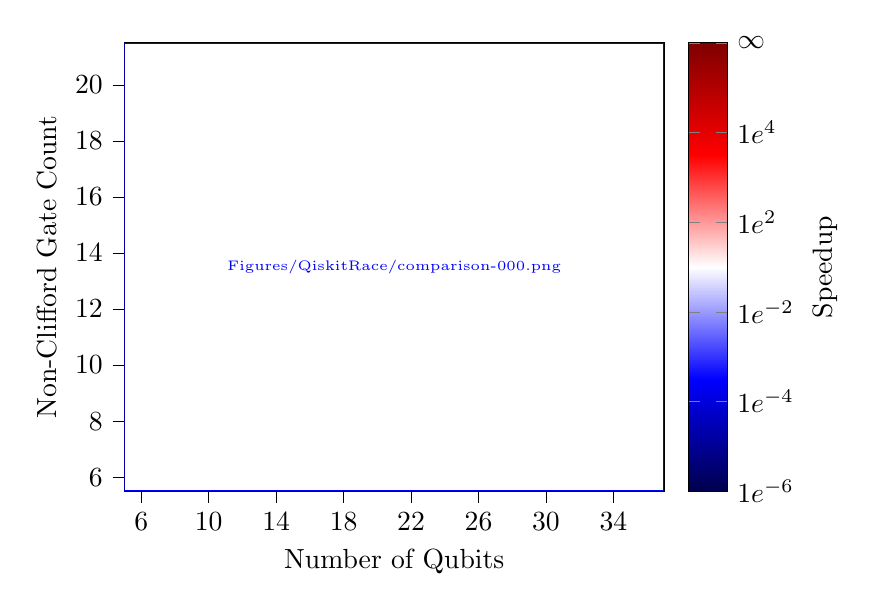
\begin{tikzpicture}

\begin{axis}[
colorbar,
colorbar style={ylabel={Speedup}, yticklabels={a,$1e^{-6}$,$1e^{-4}$,$1e^{-2}$,$1e^{2}$,$1e^{4}$,$\infty$}},
colormap={mymap}{[1pt]
  rgb(0pt)=(0,0,0.3);
  rgb(1pt)=(0,0,1);
  rgb(2pt)=(1,1,1);
  rgb(3pt)=(1,0,0);
  rgb(4pt)=(0.5,0,0)
},
point meta max=1,
point meta min=0,
tick align=outside,
tick pos=left,
x grid style={white!69.01960784313725!black},
xlabel={Number of Qubits},
xmin=-0.5, xmax=15.5,
xtick style={color=black},
xtick={0,2,4,6,8,10,12,14},
xticklabels={6,10,14,18,22,26,30,34},
y grid style={white!69.01960784313725!black},
ylabel={Non-Clifford Gate Count},
ymin=-0.5, ymax=15.5,
ytick style={color=black},
ytick={0,2,4,6,8,10,12,14},
yticklabels={6,8,10,12,14,16,18,20}
]
\addplot graphics [includegraphics cmd=\pgfimage,xmin=-0.5, xmax=15.5, ymin=15.5, ymax=-0.5] {Figures/QiskitRace/comparison-000.png};
\end{axis}

\end{tikzpicture}
\end{scaletikzpicturetowidth}
\caption{Figure comparing the runtime of stabilizer rank-based simulations to the \texttt{Qiskit} state-vector simulation for random circuits, using \texttt{Qiskit-Aer}. The solid red region corresponds to the regime where quantum circuits required too much memory to simulate with state-vector methods.}\label{fig:qiskit_race}
\end{figure}
As we can see, the runtime of the stabilizer-rank based methods increases with the number of non-Clifford gates, which we expect as the extent also increases. However, even for circuits with small extent, below $20$ qubits the stabilizer rank method requires significantly increased runtime compared to the state-vector approach.\par
As the number of qubits continues to increase, the stabilizer rank method becomes increasingly efficient. Above a hard upper limit of $30$ qubits, the spatial requirements of the state-vector simulator exceed the available memory, and so the circuits can no longer be run. The stabilizer rank simulator, however, is still capable of running the simulation. it is also important to note that, as expected, the runtime of the stabilizer state method does not increase significantly with the number of qubits. For example, a circuit on $50$ qubits and with $20$ non-Clifford gates required on average $246$ seconds to simulate with the stabilizer-rank method, compared to the $213$ seconds required by the state-vector method to simulate a similar circuit on $30$ qubits.
\subsection{Simulations of Quantum Circuits}\label{sec:circuit_simulations}
% Results of simulations performed with this method
In this section, we will present results using the stabilizer rank method to simulate three common classes of quantum circuit: `oracle' or black-box circuits, variational methods, and random circuits.
\subsubsection*{Hidden Shift Circuits}
% Used to verify the Simulator
Oracle-based circuits are a common technique for designing quantum algorithms, encompassing everything from toy methods such as the Deutsch-Jozsa algorithm up to famous algorithms like Grover search and Shor's algorithm~\cite{Mosca2008}. These methods generally involve initializing the quantum state in a superposition of computational basis states, and then applying a black-box unitary $O_{f}$ that computes some classical function $f$~\cite{Nielsen2000}.\par
The hidden-shift problem is an example of a computational task where quantum algorithms require fewer invocations or queries to the oracle than any classical method~\cite{Roetteler2008}. Consider a `bent' boolean function $f(\va{x}):\mathbb{Z}_{2}^{n}\rightarrow \pm 1$, which has the property that its Fourier coefficients $\hat{f}\left(\va{w}\right)=\frac{1}{2^{n}}\sum_{\va{x}}\left(-1\right)^{\va{w}\cdot \va{x} + f\left(\va{x}\right)}$ are equal for all $n$-bit strings $w$.\par
For any boolean function, we can also define a shifted function $f_{\va{s}}$ as $f_{\va{s}}\left(\va{x}\right)=f\left(\va{x}\oplus \va{s}\right)$, where $\va{s}\in\mathbb{Z}_{2}^{n}$ is a fixed binary string. Finally, we can also define the Fourier transformed dual of the bent function as~\cite{Roetteler2008}
\[ \tilde{f}\left(\va{x}\right) = 2^{-n/2}\sum_{\va{y}\in\mathbb{Z}_{2}^{n}}\left(-1\right)^{\va{x}\cdot \va{y}}f\left(\va{y}\right) \]
Given oracles $O_{f_{\va{s}}}$ and $O_{\tilde{f}}$ that will evaluate both the shifted function and its unshifted dual for some input string $\va{x}$, it will take a classical method $O(n)$ queries to determine the `hidden' shift string $\va{s}$. However, a quantum algorithm can determine $\va{s}$ in just two queries.
\begin{figure}[H]
\centerline{
\Qcircuit @C=1em @R=.7em {
    \lstick{\ket{0^{\otimes n}}} & \gate{H^{\otimes n}} & \gate{O_{f_{\va{s}}}} & \gate{H^{\otimes n}} & \gate{O_{\tilde{f}}} & \gate{H^{\otimes n}} & \rstick{\ket{\va{s}}} \qw \\
}}
\caption{Circuit diagram of the quantum method for solving the hidden-shift problem, described in~\cite{Roetteler2008}.}
\end{figure}
It is interesting to note that, if we further restrict this problem to only have access to $f_{\va{s}}$ and $f$, and not the dual bent function, there nonetheless exists an alternative quantum algorithm capable of solving for $\va{s}$ in $O(n)$ queries. The authors conjecture that in this case a classical method would require an exponential number of queries~\cite{Roetteler2008}.\par
The specific class of bent functions considered in~\cite{Roetteler2008} are called Majorana-McFarland functions. In practice, we can construct a quantum oracle for random bent functions from this family using a fixed number of $CCZ$ gates. This method was outlined in Appendix~F of~\cite{Bravyi2016}, which used the hidden-shift problem to benchmark the performance of the stabilizer rank simulation method. Because we specify the string $s$ in the construction of the oracle, this method has `built-in' verification that the simulator is running correctly.\par
In particular,~\cite{Bravyi2016} detail how to construct a bent function starting from a random boolean function $g:\mathbb{Z}_{2}^{n/2}\rightarrow \pm 1$, which they generate using a random sequence of $Z$ and $CZ$ gates and a fixed number of $CCZ$ gates. If we denote this circuit $O_{r}$, then the oracles for the hidden-shift problem are defined as
\begin{equation}
\begin{array}{l r}
 O_{f_{\va{s}}} = \left[\left(\prod_{i=1}^{n/2}CZ_{i,i+n/2}\right)I\otimes O_{r}\right] Z\left(\va{s}\right) & O_{\tilde{f}} = \left(\prod_{i=1}^{n/2}CZ_{i,i+n/2}\right)O_{r}\otimes I
\end{array}
\end{equation}
For $m$ $CCZ$ gates, the overall circuit thus contains $2m$ non-Clifford gates. In~\cite{Bravyi2016}, they simulate these circuits by using a gadget for $CCZ$ gates built out of $4$ $T$ gates. Here, we use the hidden-shift circuits on $40$ qubits as a way to test our results on decomposing alternate Clifford magic states, and the sum-over-Cliffords picture. In particular, we simulate the hidden-shift circuits using four distinct methods
\begin{itemize}
    \item A gadgetized decomposition, using $4$ $\ket{T}$ magic states to synthesis each $CCZ$ gate
    \item A gadgetized decomposition, using $\ket{CCZ}$ magic states directly
    \item A sum-over-Cliffords decomposition, using 4 $T$ gates per $CCZ$ gate
    \item A sum-over-Cliffords decomposition, using $CCZ$ gates
\end{itemize}
This allows us to directly compare the sum-over-Cliffords and gadgetized methods, and to compare direct decompositions with Clifford+$T$ synthesis.\par
The simulation was developed in collaboration with Mark Howard, based on the previous simulations developed by David Gosset in~\cite{Bravyi2016}. The setup for the simulation, including constructing the oracle circuits, and constructing the PBC projectors in the gadgetized method, are implemented in \texttt{MATLAB}.\par
As previously stated, sampling from $n$ output bits with the norm estimation routine has a runtime that scales as $O\left(\chi_{\epsilon}n^{6}\right)$. To circumvent this, we exploit the fact that we can clasically cache the state of the simulation before measurement, and that the output state of the simulation is an approximation of single output string $\ket{s}$, and learn the string $\va{s}$ by sampling single qubits a time. An example of this is shown in Figure~\ref{fig:hs_readout}. Overall, this method takes time $\left(\chi_{\epsilon}n^{4}\right)$ to sample from all $n$ bits.\par
\begin{figure}[t]
\centering
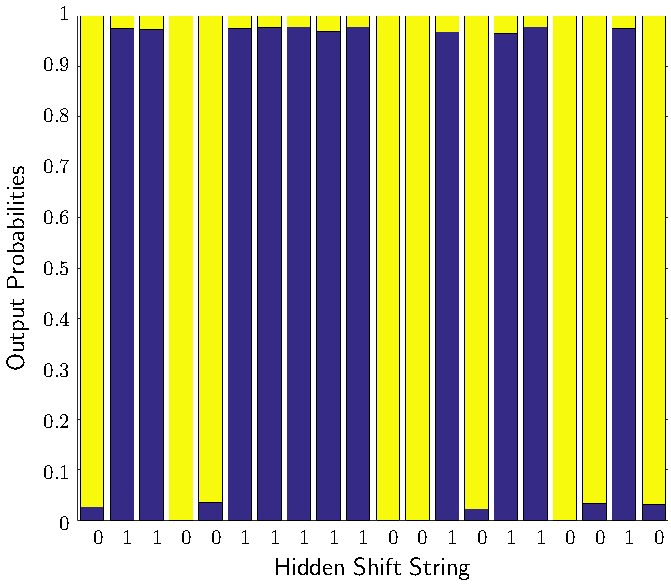
\includegraphics[width=0.75\textwidth]{Figures/HiddenShiftHistogram.pdf}
\caption{Figure showing the probability $P\left(x_{i}=1\right)$ for $20$ bits, obtained using the sum-over-Cliffords methods and synthesizing the $CCZ$ gate with $4$ $T$ gates. Each output probability is computed individually.}
\label{fig:hs_readout}
\end{figure}
To cache the decomposition between each norm estimation step, we store the choice of subspace or Clifford branches in MATLAB. We then make use of the \texttt{MEX} API to pass this data, and the Pauli projectors to be applied, to the \texttt{C++} simulator. This computes and returns the probability $p_{x_{i}=1}$, and we then sample bits by generating uniform random numbers $r\in [0,1)$ and returning $1$ iff $r<p_{x_{i}=1}$.\par
In the gadgetized case, the number of terms in the decomposition depends on the stabilizer fidelity and the target infidelity, which we will denote here as $\Delta$. Using the stabilizer fidelity of the $\ket{T}$ and $\ket{CCZ}$, then for a bent function using $m$ $CCZ$ gates the size of the decomposition $\chi$ scales as
\begin{equation}
\begin{array}{l r}
F\left(T\right)\approx 0.853 & \chi = \lfloor\frac{4 F\left(T\right)^{-8m}}{\Delta}\rfloor \approx \lfloor 4\left(\frac{3.57^{m}}{\Delta}\right)\rfloor\\ 
F\left(CCZ\right)\approx \frac{9}{16} & \chi = \lfloor\frac{4 F\left(CCZ\right)^{-2m}}{\Delta}\rfloor \approx \lfloor 4\left(\frac{3.16^{m}}{\Delta}\right)\rfloor\\ 
\end{array}
\end{equation}
Similarly, for the sum-over-Cliffords method, the number of terms is given by the stabilizer extent, and the target error $\epsilon$. For $m$ $CCZ$ gates, the number of terms is given by
\begin{equation}
\begin{array}{l r}
\xi\left(T\right) \approx 1.17 & \chi = \lceil 1.17^{8m} \epsilon^{-2}\rceil = \lceil 3.57^{m}\epsilon^{-2}\rceil \\
\xi\left(CCZ\right) = \frac{16}{9} & \chi = \lceil 1.78^{2m}\epsilon^{-2}\rceil = \lceil 3.16^{m}\epsilon^{-2}\rceil
\end{array}
\end{equation}
Recall that for Clifford magic states, the stabilizer fidelity and stabilizer extent coincide, which explains the correspondence in the scaling between the random codes and sum-over-Cliffords method. In all the simulations, we set $\Delta=\epsilon=0.3$. Due to platform limitations, the \texttt{C++} component was executed serially, though decompositions were built in parallel using \texttt{MATLAB}'s built in parallel execution. All simulations were run on a dual-core $1.9\mathrm{GHz}$ Intel Xeon, with $32\mathrm{GB}$ of RAM.\ The results are shown in Figure~\ref{fig:hs_results}.
\begin{figure}[t]
\centering
\caption{Figures demonstrating the performance of the stabilizer rank method on simulating the hidden shift problem, using $4$ methods of building the stabilizer state decomposition. Figures originally created for~\cite{Bravyi2018}}\label{fig:hs_results}
\begin{subfigure}[t]{0.45\textwidth}
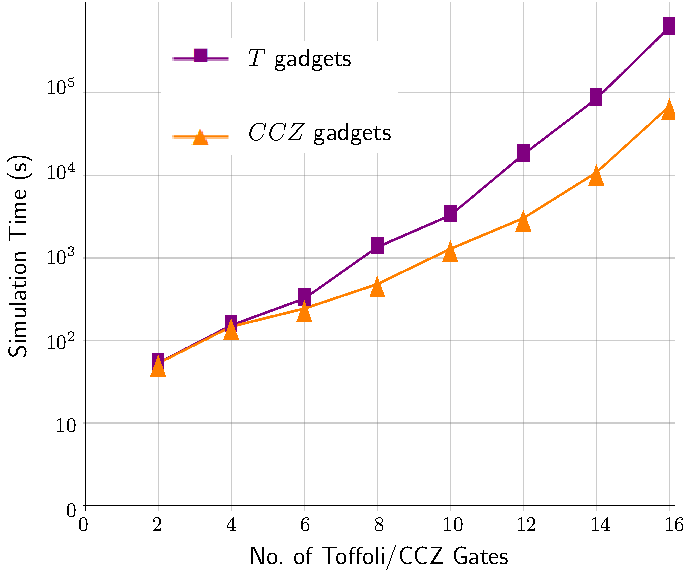
\includegraphics[width=\textwidth]{HiddenShiftTimes_RC.pdf}
\caption{Runtime of the hidden shift simulation as a function of the number of $CCZ$ gates, using the random codes method to build decompositions, using Clifford+$T$ synthesis and direct decomposition.}\label{fig:hs_rc_times}
\vspace{2cm}
\end{subfigure}
\begin{subfigure}[t]{0.45\textwidth}
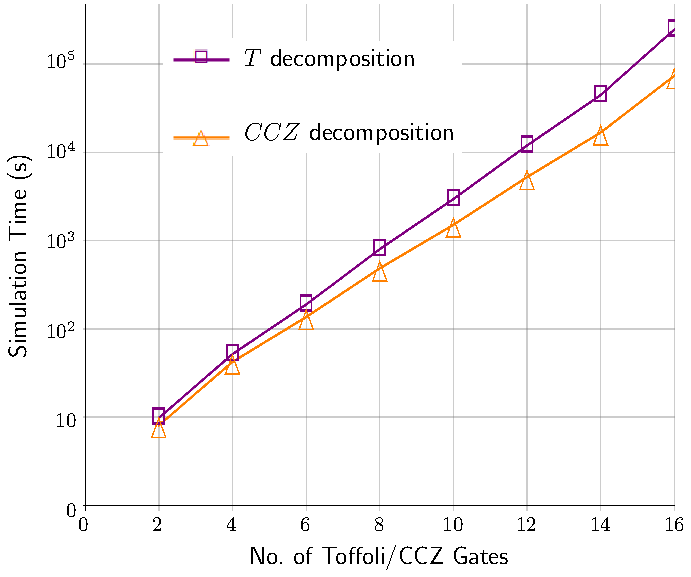
\includegraphics[width=\textwidth]{Figures/HiddenShiftTimes_SoC.pdf}
\caption{Runtime of the hidden shift simulation as a function of the number of $CCZ$ gates, using the sum-over-Cliffords method to build decompositions, comparing Clifford+$T$ synthesis with $CCZ$ gates.}\label{fig:hs_sc_times}
\end{subfigure}
% \end{figure}
% \begin{figure}[H]\ContinuedFloat
\begin{subfigure}[t]{0.6\textwidth}
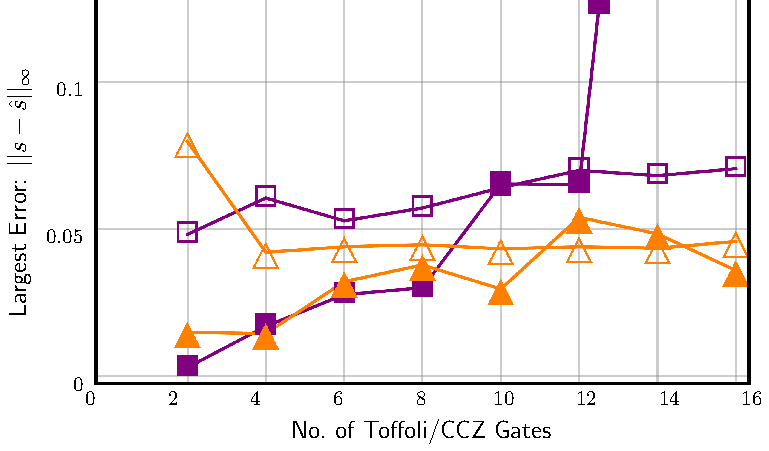
\includegraphics[width=\textwidth]{Figures/HiddenShiftErrors.pdf}
\caption{The maximum observed approximation error in single-qubit probabilities over all bits in the hidden-shift string. The colour and markers correspond to the timing plots above. Not shown are two data-points in the $T$ random-code methods, for $14$ and $16$ Toffoli gates, with large errors $0.304$ and $0.512$ respectively.}
\end{subfigure}
\end{figure}
\subsubsection*{QAOA}
As mentioned in Section~\ref{sec:simulator_intro}, current NISQ computers lack full error correction and thus accumulate noise as the circuit depth increases. Thus, there is a great deal of interest in relatively low-depth quantum algorithms that can run on NISQ devices. The main class of these algorithms are `variational methods', hybrid quantum-classical algorithms with applications in optimization and quantum computational chemistry~\cite{Moll2018}.\par
In general, variational methods use a simple processing scheme where the quantum computer is used to prepare an `ansatz' state using a low-depth circuit. The gates in the circuit are typically parameterized. We then perform a series of measurements, and these outcomes are post-processed by a classical algorithm. This can be iterated, where the parameters of the ansatz state are updated by the classical algorithm, to converge to a heuristic solution~\cite{Moll2018,Preskill2018}.\par
The Quantum Approximate Optimization Algorithm (QAOA) is an example of a variational method, applied to classical combinatorial optimization problems~\cite{Farhi2014}. These kind of optimization problems are usually specified by a number of boolean clauses, and we are interested in optimizing a function `satisfied clauses'
\[C\left(\va{z}\right) = \sum_{\alpha} C_{\alpha}\left(\va{z}\right),\]
where each sub-clause $C_{\alpha}$ acts on a subset of bits from the full $n$-bit string $\va{z}$, and evaluates to either $\{0,1\}$ or $\pm 1$ depending on the definition of the problem~\cite{Farhi2014}. A clause is said to be `satisfied' if it evaluates to $1$. Examples of combinatorial optimization problems include \textsc{MaxSat}, where we are tasked with finding the string $\va{z}$ that satisfies the most clauses simultaneously.\par
Given a clause $C_{\alpha}$, we can define an operator $\hat{C}_{\alpha}$ by replacing the bits $z_{\alpha_{i}}$ in the clause with Pauli $Z$ operators, and in turn we can define $\hat{C}=\sum_{\alpha}\hat{C}_{\alpha}$~\cite{Farhi2014}. Different computational basis strings are eigenstates of this operator, such that 
\[\hat{C}\ket{\va{z}}=C\left(\va{z}\right)\ket{\va{z}}.\]
The QAOA algorithm proceeds by preparing an ansatz state parameterized by $2p$ angles $\beta_{i}$ and $\gamma_{i}$, for some fixed value of $p$. The system is initialized in the ground state $\ket{g}$ of the operator $\hat{C}$, which depends on the definition of the problem but is typically a trivial assignment such as $\ket{0^{\otimes n}}$ or $\ket{+^{\otimes n}}$~\cite{Farhi2014,Farhi2014b}. We then apply $p$ rounds of a pair of parameterised rotation operators
\[\begin{array}{lr}
U_{C}\left(\gamma_{i}\right)=\mathe^{-\mathi \gamma \hat{C}} &  U_{B}\left(\beta_{i}\right) = \prod_{j}\mathe^{\mathi\beta_{i} X(\va{e}_{j})}
\end{array}.\]
For each paramaterised sate 
\[\ket{\psi_{\va{\gamma},\va{\beta}}}=\prod_{i=1}^{\p}\left(U_{B}\left(\beta_{i}\right)U_{C}\left(\gamma_{i}\right)\right)\ket{g}\]
has been prepared, we then perform measurements to determine the expectation value of the $\hat{C}$ operator 
\[E_{\va{\gamma},\va{\beta}}=\matrixel{\psi_{\va{\gamma},\va{\beta}}}{\hat{C}}{\psi_{\va{\gamma},\va{\beta}}}.\]
Importantly, it can be shown that as $p\rightarrow \infty$, the maximum of this expectation value corresponds to the maximum of $C\left(\va{z}\right)$~\cite{Farhi2014}. The authors further show that even with $p=1$, reasonable results that some classical strategies can be obtained~\cite{Farhi2014,Farhi2014b}.\par
We consider the application of QAOA to a combinatorial optimization problem called \textsc{MaxE3Lin2}, where QAOA has been shown to outperform random classical guesses at $p=1$~\cite{Farhi2014b}. In particular, we consider randomly generated instances of \textsc{MaxE3Lin2} with $50$ variables and $66$ clauses, requiring $50$ qubits and $66$ Pauli $Z$ rotations.\par
\begin{figure}[t]
\centering
\begin{scaletikzpicturetowidth}{0.65\textwidth}
% This file was created by matlab2tikz.
%
%The latest updates can be retrieved from
%  http://www.mathworks.com/matlabcentral/fileexchange/22022-matlab2tikz-matlab2tikz
%where you can also make suggestions and rate matlab2tikz.
%
\begin{tikzpicture}[scale=\tikzscale]

\begin{axis}[%
width=5.439in,
height=4.751in,
at={(0.912in,0.644in)},
scale only axis,
point meta min=-11.5984103084688,
point meta max=11.5984103084688,
axis on top,
xmin=-0.50125,
xmax=0.50125,
xtick={-0.5, -0.4, -0.3, -0.2, -0.1,    0,  0.1,  0.2,  0.3,  0.4,  0.5},
xlabel style={font=\color{white!15!black}},
xlabel={$\gamma\text{/}\pi$},
y dir=reverse,
ymin=-0.0025,
ymax=0.5025,
ytick={  0, 0.1, 0.2, 0.3, 0.4, 0.5},
ylabel style={font=\color{white!15!black}},
ylabel={$\beta\text{/}\pi$},
axis background/.style={fill=white},
legend style={legend cell align=left, align=left, draw=white!15!black},
colormap={mymap}{[1pt] rgb(0pt)=(0.2422,0.1504,0.6603); rgb(1pt)=(0.25039,0.164995,0.707614); rgb(2pt)=(0.257771,0.181781,0.751138); rgb(3pt)=(0.264729,0.197757,0.795214); rgb(4pt)=(0.270648,0.214676,0.836371); rgb(5pt)=(0.275114,0.234238,0.870986); rgb(6pt)=(0.2783,0.255871,0.899071); rgb(7pt)=(0.280333,0.278233,0.9221); rgb(8pt)=(0.281338,0.300595,0.941376); rgb(9pt)=(0.281014,0.322757,0.957886); rgb(10pt)=(0.279467,0.344671,0.971676); rgb(11pt)=(0.275971,0.366681,0.982905); rgb(12pt)=(0.269914,0.3892,0.9906); rgb(13pt)=(0.260243,0.412329,0.995157); rgb(14pt)=(0.244033,0.435833,0.998833); rgb(15pt)=(0.220643,0.460257,0.997286); rgb(16pt)=(0.196333,0.484719,0.989152); rgb(17pt)=(0.183405,0.507371,0.979795); rgb(18pt)=(0.178643,0.528857,0.968157); rgb(19pt)=(0.176438,0.549905,0.952019); rgb(20pt)=(0.168743,0.570262,0.935871); rgb(21pt)=(0.154,0.5902,0.9218); rgb(22pt)=(0.146029,0.609119,0.907857); rgb(23pt)=(0.138024,0.627629,0.89729); rgb(24pt)=(0.124814,0.645929,0.888343); rgb(25pt)=(0.111252,0.6635,0.876314); rgb(26pt)=(0.0952095,0.679829,0.859781); rgb(27pt)=(0.0688714,0.694771,0.839357); rgb(28pt)=(0.0296667,0.708167,0.816333); rgb(29pt)=(0.00357143,0.720267,0.7917); rgb(30pt)=(0.00665714,0.731214,0.766014); rgb(31pt)=(0.0433286,0.741095,0.73941); rgb(32pt)=(0.0963952,0.75,0.712038); rgb(33pt)=(0.140771,0.7584,0.684157); rgb(34pt)=(0.1717,0.766962,0.655443); rgb(35pt)=(0.193767,0.775767,0.6251); rgb(36pt)=(0.216086,0.7843,0.5923); rgb(37pt)=(0.246957,0.791795,0.556743); rgb(38pt)=(0.290614,0.79729,0.518829); rgb(39pt)=(0.340643,0.8008,0.478857); rgb(40pt)=(0.3909,0.802871,0.435448); rgb(41pt)=(0.445629,0.802419,0.390919); rgb(42pt)=(0.5044,0.7993,0.348); rgb(43pt)=(0.561562,0.794233,0.304481); rgb(44pt)=(0.617395,0.787619,0.261238); rgb(45pt)=(0.671986,0.779271,0.2227); rgb(46pt)=(0.7242,0.769843,0.191029); rgb(47pt)=(0.773833,0.759805,0.16461); rgb(48pt)=(0.820314,0.749814,0.153529); rgb(49pt)=(0.863433,0.7406,0.159633); rgb(50pt)=(0.903543,0.733029,0.177414); rgb(51pt)=(0.939257,0.728786,0.209957); rgb(52pt)=(0.972757,0.729771,0.239443); rgb(53pt)=(0.995648,0.743371,0.237148); rgb(54pt)=(0.996986,0.765857,0.219943); rgb(55pt)=(0.995205,0.789252,0.202762); rgb(56pt)=(0.9892,0.813567,0.188533); rgb(57pt)=(0.978629,0.838629,0.176557); rgb(58pt)=(0.967648,0.8639,0.16429); rgb(59pt)=(0.96101,0.889019,0.153676); rgb(60pt)=(0.959671,0.913457,0.142257); rgb(61pt)=(0.962795,0.937338,0.12651); rgb(62pt)=(0.969114,0.960629,0.106362); rgb(63pt)=(0.9769,0.9839,0.0805)},
colorbar
]
\addplot [forget plot] graphics [xmin=-0.50125, xmax=0.50125, ymin=-0.0025, ymax=0.5025] {QAOA/MCPlot-1.png};
\end{axis}
\end{tikzpicture}%
\end{scaletikzpicturetowidth}
\caption{Heat-map showing the expectation value $E_{\beta,\gamma}$ for the simulated instance of \textsc{MaxE3Lin2}, generated using the method of~\cite{VandenNest2009}, implemented in \texttt{MATLAB}.}\label{fig:mc_qaoa}
\end{figure}
The goal of \textsc{MaxE3Lin2} is to maximize an objective-function
\[C\left(\va{z}\right) = \frac{1}{2}\sum_{1\leq u < v < w \leq n} d_{uvw}z_{u}z_{v}z_{w}\]
where each clause acts on $3$ variables~\cite{Farhi2014b,Bravyi2018}, and the coefficients $d_{uvw}=\{0,\pm1\}$. The number of clauses is given by the number of non-zero coefficients. When generating the problems, restrict ourselves to instances with fixed degree $4$, such that each qubit appears in at most $4$ terms. We then prepare a state 
\[\ket{\psi_{\gamma,\beta}} = U_{B}\left(\beta\right)U_{C}\left(\gamma\right)\ket{+^{\otimes n}}\]
with two parameters~\cite{Farhi2014b}.\par
Classical preprocessing methods exist for estimating $E_{\gamma,\beta}$, which can be used to speed-up the classical step of the variational algorithm. In particular, we use a method that allows the expectation variables of a sparse Hamiltonian with `computationally tractable' states, states which can be efficiently specified in the computational basis~\cite{VandenNest2009}. This allows us to approximately compute
\[\matrixel{\psi_{\gamma}}{U_{B}\left(\beta\right)^{\dagger} \hat{C}U_{B}\left(\beta\right)}{\psi_{\gamma}}\]
with additive error $\epsilon$ in time $O(m^{4}\epsilon^{-2})$~\cite{Bravyi2018}. Figure~\ref{fig:mc_qaoa} plots the estimates of $E_{\gamma,\beta}$ for a particular instance of \textsc{MaxE3Lin2}.\par
In their original paper, Farhi et al.\ fix $\beta=\pi/4$. This has the advantage that the rotation $U_{B}$ becomes a Clifford operator 
\[\mathe^{-\mathi \pi/4 X\left(\va{e}_{i}\right)}=H\left(\va{e}_{i}\right)S\left(\va{e}_{i}\right)H\left(\va{e}_{i}\right),\]
meaning all non-Clifford terms arise from the $Z$ rotations. We can also see from Figure~\ref{fig:mc_qaoa} that the line from $\beta=\pi/4$ passes through a local minima and maxima of $C\left(\va{z}\right)$. Thus, in our simulation, we also fix $\beta=\pi/4$. The cost function is antisymmetric about $\gamma=0$, and so we sweep $\gamma$ from $0$ to $\pi$.\par
Each rotation in $U_{C}$ has a sum-over-Cliffords expansion~\cite{Bravyi2018}
\[\mathe^{-\mathi \frac{\gamma}{2} d_{uvw}Z_{u}Z_{v}Z_{w}} = \begin{cases}
\alpha I + \beta CNOT_{u,v}CZ_{v,w}S_{v}S_{w}CNOT_{u,v} & d_{uvw} = 1\\
\alpha I + \beta \mathi CNOT_{u,v}CZ_{v,w}S^{\dagger}_{v}S^{\dagger}_{w}CNOT_{u,v} & d_{uvw} = -1\\
\end{cases}\]
where the coefficients $\alpha$ and $\beta$ are the phase terms associated with each branch
\[\begin{array}{lr}
b_{0} = \mathe^{\mathi \gamma}-\mathi & \alpha = \frac{b_{0}}{\left|b_{0}\right|}\\
b_{1} = 1 - \mathe^{\mathi \gamma} & \beta = \frac{b_{1}}{\left|b_{1}\right|}\\
\end{array}.\]
For each value of $\gamma$, we build the corresponding stabilizer state decomposition with
\[\chi = \lceil \xi\left(\gamma\right)\epsilon^{-2}\rceil = \lceil \left(\left|b_{0}\right|+\left|b_{1}\right|\right)^{2m}\epsilon^{-2}\rceil \]
terms for $m$ clauses. We then run the Metropolis method to take $40000$ samples from the output distribution of the state $\ket{\psi_{\gamma}}$, and compute an estimate of the expectation value
\begin{equation}
E_{sim}\left(\gamma\right)\frac{1}{40000}\sum_{s=1}^{40000}C\left(z_{s}\right).
\end{equation}
The simulations were run on the UCL Legion supercomputing cluster, running on Dell C6100 compute nodes, using a shared-memory parallelism model with $12$ parallel threads and $24\mathrm{GB}$ of RAM.\ We ran these methods with $\epsilon=0.1$ and $0.15$, and compare our estimates to the results from the heuristic method of~\cite{VandenNest2009}. Results are shown in Figure~\ref{fig:qaoa_results}.
\begin{figure}[H]
\centering
\begin{subfigure}[t]{0.7\textwidth}
\begin{scaletikzpicturetowidth}{\textwidth}
% This file was created by matlab2tikz.
%
%The latest updates can be retrieved from
%  http://www.mathworks.com/matlabcentral/fileexchange/22022-matlab2tikz-matlab2tikz
%where you can also make suggestions and rate matlab2tikz.
%
\definecolor{mycolor1}{rgb}{0.00000,0.44700,0.74100}%
\definecolor{mycolor2}{rgb}{0.85000,0.32500,0.09800}%
%
\begin{tikzpicture}[scale=\tikzscale]

\begin{axis}[%
width=6.028in,
height=4.567in,
at={(1.011in,0.829in)},
scale only axis,
xmin=0,
xmax=0.5,
xlabel style={font=\color{white!15!black}},
xlabel={$2\gamma\text{/}\pi$},
ymin=-8,
ymax=2,
ylabel style={font=\color{white!15!black}},
ylabel={E3LIN2 Cost function},
axis background/.style={fill=white},
axis x line*=bottom,
axis y line*=left,
legend style={at={(0.97,0.03)}, anchor=south east, legend cell align=left, align=left, draw=white!15!black}
]
\addplot [color=black, draw=none, mark=asterisk, mark options={solid, black}]
  table[row sep=crcr]{%
0	7.23766258296095e-19\\
0.005	-0.517387795912572\\
0.01	-1.03146943864507\\
0.015	-1.53897192228841\\
0.02	-2.03668809890773\\
0.025	-2.52150852346372\\
0.03	-2.99045201726915\\
0.035	-3.44069455350371\\
0.04	-3.8695960969761\\
0.045	-4.27472505987768\\
0.05	-4.65388007301621\\
0.055	-5.00510881841644\\
0.06	-5.32672370200259\\
0.065	-5.61731421223962\\
0.07	-5.87575584208564\\
0.075	-6.10121551541453\\
0.08	-6.29315350830479\\
0.085	-6.45132190117333\\
0.09	-6.5757596578082\\
0.095	-6.66678446477068\\
0.1	-6.72498151759582\\
0.105	-6.75118947283254\\
0.11	-6.74648382883177\\
0.115	-6.71215802748821\\
0.12	-6.64970258922686\\
0.125	-6.56078262437271\\
0.13	-6.44721407038408\\
0.135	-6.31093901566185\\
0.14	-6.15400047317911\\
0.145	-5.97851696397588\\
0.15	-5.78665725899553\\
0.155	-5.58061561815934\\
0.16	-5.36258783682975\\
0.165	-5.13474839752925\\
0.17	-4.8992289871885\\
0.175	-4.65809861250893\\
0.18	-4.41334551177191\\
0.185	-4.16686102562392\\
0.19	-3.92042555376292\\
0.195	-3.67569667918891\\
0.2	-3.43419951695323\\
0.205	-3.19731929385976\\
0.21	-2.96629614100135\\
0.215	-2.74222204076003\\
0.22	-2.52603984288623\\
0.225	-2.31854423439293\\
0.23	-2.12038452615348\\
0.235	-1.93206909443026\\
0.24	-1.7539713034495\\
0.245	-1.5863367180089\\
0.25	-1.42929140959061\\
0.255	-1.28285115272387\\
0.26	-1.14693130784651\\
0.265	-1.02135719035564\\
0.27	-0.905874731019478\\
0.275	-0.800161242858236\\
0.28	-0.703836120396919\\
0.285	-0.616471313973611\\
0.29	-0.537601435772637\\
0.295	-0.466733373186167\\
0.3	-0.403355304213919\\
0.305	-0.346945028589206\\
0.31	-0.296977547776855\\
0.315	-0.252931846967565\\
0.32	-0.214296850253144\\
0.325	-0.180576538153512\\
0.33	-0.151294233078071\\
0.335	-0.12599607295437\\
0.34	-0.104253706747664\\
0.345	-0.0856662563199942\\
0.35	-0.0698615988512662\\
0.355	-0.0564970308508585\\
0.36	-0.0452593802473119\\
0.365	-0.0358646361550923\\
0.37	-0.028057167399935\\
0.375	-0.0216086004819897\\
0.38	-0.0163164258628945\\
0.385	-0.0120023981302957\\
0.39	-0.00851079131618697\\
0.395	-0.00570656527837396\\
0.4	-0.00347349313137661\\
0.405	-0.00171229323744115\\
0.41	-0.000338802616529245\\
0.415	0.000717778082813723\\
0.42	0.00151654445388408\\
0.425	0.00210643568093258\\
0.43	0.0025276577681041\\
0.435	0.00281297624774502\\
0.44	0.00298887651385709\\
0.445	0.00307659376481914\\
0.45	0.00309301765781979\\
0.455	0.00305147917214302\\
0.46	0.00296242888960545\\
0.465	0.00283401697355533\\
0.47	0.00267258564612329\\
0.475	0.0024830850032192\\
0.48	0.002269422675762\\
0.485	0.00203475724017241\\
0.49	0.00178174450851599\\
0.495	0.00151274498985604\\
0.5	0.00123\\
};
\addlegendentry{Van den Nest}

\addplot [color=red, draw=none, mark=square*, mark options={solid, red,fill=red!80!black}]
  table[row sep=crcr]{%
0	-0.0422666666666667\\
0.0159154943091895	-1.5052\\
0.0318309886183791	-2.9941\\
0.0477464829275686	-4.51186666666667\\
0.0636619772367581	-5.3909\\
0.0795774715459477	-6.28516666666667\\
0.0954929658551372	-6.36753333333333\\
0.111408460164327	-6.70043333333333\\
0.127323954473516	-6.18606666666667\\
0.143239448782706	-6.13003333333333\\
0.159154943091895	-5.36216666666667\\
0.175070437401085	-4.63116666666667\\
0.190985931710274	-3.51306666666667\\
0.206901426019464	-3.1699\\
0.222816920328653	-2.53586666666667\\
0.238732414637843	-1.8411\\
0.254647908947033	-1.1805\\
0.270563403256222	-0.9637\\
0.286478897565412	-0.451633333333333\\
0.302394391874601	-0.569833333333333\\
0.318309886183791	-0.145666666666667\\
0.33422538049298	0.00173333333333333\\
0.35014087480217	-0.1569\\
0.366056369111359	0.3096\\
0.381971863420549	-0.0915333333333333\\
0.397887357729738	0.142133333333333\\
0.413802852038928	-0.0644333333333333\\
0.429718346348117	-0.0240666666666667\\
0.445633840657307	-0.2141\\
0.461549334966496	-0.220066666666667\\
0.477464829275686	0.0268\\
};
\addlegendentry{$\text{Sum-over-Cliffords, }\epsilon\text{=0.1}$}

\addplot [color=blue, draw=none, mark=square*, mark options={solid, blue, fill=blue!80!black}]
  table[row sep=crcr]{%
0	-0.0218\\
0.0159154943091895	-1.747\\
0.0318309886183791	-3.02526666666667\\
0.0477464829275686	-4.35733333333333\\
0.0636619772367581	-5.41123333333333\\
0.0795774715459477	-6.26973333333333\\
0.0954929658551372	-6.97373333333333\\
0.111408460164327	-6.4866\\
0.127323954473516	-6.63696666666667\\
0.143239448782706	-6.2095\\
0.159154943091895	-5.3887\\
0.175070437401085	-4.43733333333333\\
0.190985931710274	-4.0434\\
0.206901426019464	-3.22253333333333\\
0.222816920328653	-2.39756666666667\\
0.238732414637843	-1.52216666666667\\
0.254647908947033	-0.840166666666667\\
0.270563403256222	-1.1053\\
0.286478897565412	-0.652533333333333\\
0.302394391874601	-0.6133\\
0.318309886183791	-0.333633333333333\\
0.33422538049298	-0.0962\\
0.35014087480217	-0.1399\\
0.366056369111359	-0.2656\\
0.381971863420549	0.0272333333333333\\
0.397887357729738	0.0181\\
0.413802852038928	-0.123633333333333\\
0.429718346348117	-0.1615\\
0.445633840657307	-0.0860333333333333\\
0.461549334966496	-0.0111666666666667\\
0.477464829275686	-0.606333333333333\\
};
\addlegendentry{$\text{Sum-over-Cliffords, }\epsilon\text{=0.15}$}

\addplot [color=mycolor1, draw=none, forget plot]
 plot [error bars/.cd, y dir = both, y explicit]
 table[row sep=crcr, y error plus index=2, y error minus index=3]{%
0	-0.0218	0.0986987781542364	0.0986987781542364\\
0.0159154943091895	-1.747	0.101609649763234	0.101609649763234\\
0.0318309886183791	-3.02526666666667	0.100062545868425	0.100062545868425\\
0.0477464829275686	-4.35733333333333	0.102145521130549	0.102145521130549\\
0.0636619772367581	-5.41123333333333	0.10707737997756	0.10707737997756\\
0.0795774715459477	-6.26973333333333	0.12501319208995	0.12501319208995\\
0.0954929658551372	-6.97373333333333	0.115827934371132	0.115827934371132\\
0.111408460164327	-6.4866	0.147055561408474	0.147055561408474\\
0.127323954473516	-6.63696666666667	0.15850459733756	0.15850459733756\\
0.143239448782706	-6.2095	0.189562231537889	0.189562231537889\\
0.159154943091895	-5.3887	0.189618321191351	0.189618321191351\\
0.175070437401085	-4.43733333333333	0.19280984997055	0.19280984997055\\
0.190985931710274	-4.0434	0.192470954468784	0.192470954468784\\
0.206901426019464	-3.22253333333333	0.210756609441615	0.210756609441615\\
0.222816920328653	-2.39756666666667	0.190582218491314	0.190582218491314\\
0.238732414637843	-1.52216666666667	0.184705268416975	0.184705268416975\\
0.254647908947033	-0.840166666666667	0.165929816030142	0.165929816030142\\
0.270563403256222	-1.1053	0.189051353481152	0.189051353481152\\
0.286478897565412	-0.652533333333333	0.168953403255994	0.168953403255994\\
0.302394391874601	-0.6133	0.177770676819516	0.177770676819516\\
0.318309886183791	-0.333633333333333	0.181408446150672	0.181408446150672\\
0.33422538049298	-0.0962	0.172462152903636	0.172462152903636\\
0.35014087480217	-0.1399	0.15421615689723	0.15421615689723\\
0.366056369111359	-0.2656	0.173664087015585	0.173664087015585\\
0.381971863420549	0.0272333333333333	0.167973521588758	0.167973521588758\\
0.397887357729738	0.0181	0.18889657268075	0.18889657268075\\
0.413802852038928	-0.123633333333333	0.13869218905879	0.13869218905879\\
0.429718346348117	-0.1615	0.150222758224405	0.150222758224405\\
0.445633840657307	-0.0860333333333333	0.170192984997663	0.170192984997663\\
0.461549334966496	-0.0111666666666667	0.181262138921885	0.181262138921885\\
0.477464829275686	-0.606333333333333	0.269343907836675	0.269343907836675\\
};
\addplot [color=mycolor2, draw=none, forget plot]
 plot [error bars/.cd, y dir = both, y explicit]
 table[row sep=crcr, y error plus index=2, y error minus index=3]{%
0	-0.0422666666666667	0.0884411398131475	0.0884411398131475\\
0.0159154943091895	-1.5052	0.104223310560919	0.104223310560919\\
0.0318309886183791	-2.9941	0.0995473858448632	0.0995473858448632\\
0.0477464829275686	-4.51186666666667	0.108259293811696	0.108259293811696\\
0.0636619772367581	-5.3909	0.10892092075721	0.10892092075721\\
0.0795774715459477	-6.28516666666667	0.120881119711588	0.120881119711588\\
0.0954929658551372	-6.36753333333333	0.169797948210377	0.169797948210377\\
0.111408460164327	-6.70043333333333	0.13533915340608	0.13533915340608\\
0.127323954473516	-6.18606666666667	0.176379947879713	0.176379947879713\\
0.143239448782706	-6.13003333333333	0.163345775987938	0.163345775987938\\
0.159154943091895	-5.36216666666667	0.199806558325872	0.199806558325872\\
0.175070437401085	-4.63116666666667	0.202306424138162	0.202306424138162\\
0.190985931710274	-3.51306666666667	0.188568424166203	0.188568424166203\\
0.206901426019464	-3.1699	0.177214689651149	0.177214689651149\\
0.222816920328653	-2.53586666666667	0.184935476755038	0.184935476755038\\
0.238732414637843	-1.8411	0.175876471486551	0.175876471486551\\
0.254647908947033	-1.1805	0.161635689104699	0.161635689104699\\
0.270563403256222	-0.9637	0.172991169578456	0.172991169578456\\
0.286478897565412	-0.451633333333333	0.165947642438498	0.165947642438498\\
0.302394391874601	-0.569833333333333	0.183996662805418	0.183996662805418\\
0.318309886183791	-0.145666666666667	0.17074695250335	0.17074695250335\\
0.33422538049298	0.00173333333333333	0.162425975206599	0.162425975206599\\
0.35014087480217	-0.1569	0.166734662076444	0.166734662076444\\
0.366056369111359	0.3096	0.173518296462775	0.173518296462775\\
0.381971863420549	-0.0915333333333333	0.162164364024179	0.162164364024179\\
0.397887357729738	0.142133333333333	0.151443001361364	0.151443001361364\\
0.413802852038928	-0.0644333333333333	0.156521699214936	0.156521699214936\\
0.429718346348117	-0.0240666666666667	0.171686028231559	0.171686028231559\\
0.445633840657307	-0.2141	0.182471868300435	0.182471868300435\\
0.461549334966496	-0.220066666666667	0.222785336054746	0.222785336054746\\
0.477464829275686	0.0268	0.222378600117461	0.222378600117461\\
};
\end{axis}
\end{tikzpicture}%
\end{scaletikzpicturetowidth}
\caption{Plot comparing the estimates of $E_{\gamma}$ obtained using the methods of~\cite{VandenNest2009}, with the estimates obtained using the sum-over-Cliffords simulator and sampling from the output distribution with the Metropolis method.}\label{fig:qaoa_results_comparison}
\end{subfigure}
\begin{subfigure}[t]{0.7\textwidth}
\begin{scaletikzpicturetowidth}{\textwidth}
% This file was created by matlab2tikz.
%
%The latest updates can be retrieved from
%  http://www.mathworks.com/matlabcentral/fileexchange/22022-matlab2tikz-matlab2tikz
%where you can also make suggestions and rate matlab2tikz.
%
\begin{tikzpicture}[scale=\tikzscale]

\begin{axis}[%
width=6.028in,
height=4.567in,
at={(1.011in,0.829in)},
scale only axis,
xmin=0,
xmax=0.5,
xlabel style={font=\color{white!15!black}},
xlabel={$\gamma\text{/}\pi$},
ymin=0,
ymax=3500000,
ylabel style={font=\color{white!15!black}},
ylabel={Number of Stabilizer States},
axis background/.style={fill=white},
axis x line*=bottom,
axis y line*=left,
legend style={legend cell align=left, align=left, draw=white!15!black}
]
\addplot [color=red, draw=none, mark=asterisk, mark options={solid, red}]
  table[row sep=crcr]{%
0	100\\
0.0159154943091895	374\\
0.0318309886183791	1272\\
0.0477464829275686	3942\\
0.0636619772367581	11149\\
0.0795774715459477	28818\\
0.0954929658551372	68168\\
0.111408460164327	147729\\
0.127323954473516	293606\\
0.143239448782706	535632\\
0.159154943091895	897653\\
0.175070437401085	1382858\\
0.190985931710274	1959352\\
0.206901426019464	2554493\\
0.222816920328653	3065484\\
0.238732414637843	3386842\\
0.254647908947033	3445455\\
0.270563403256222	3227478\\
0.286478897565412	2783617\\
0.302394391874601	2210064\\
0.318309886183791	1614816\\
0.33422538049298	1085407\\
0.35014087480217	670802\\
0.366056369111359	380944\\
0.381971863420549	198645\\
0.397887357729738	95033\\
0.413802852038928	41671\\
0.429718346348117	16730\\
0.445633840657307	6142\\
0.461549334966496	2059\\
0.477464829275686	630\\
};
\addlegendentry{$\epsilon\text{=0.1}$}

\addplot [color=blue, draw=none, mark=asterisk, mark options={solid, blue}]
  table[row sep=crcr]{%
0	45\\
0.0159154943091895	167\\
0.0318309886183791	566\\
0.0477464829275686	1752\\
0.0636619772367581	4955\\
0.0795774715459477	12808\\
0.0954929658551372	30297\\
0.111408460164327	65658\\
0.127323954473516	130492\\
0.143239448782706	238059\\
0.159154943091895	398957\\
0.175070437401085	614604\\
0.190985931710274	870824\\
0.206901426019464	1135330\\
0.222816920328653	1362437\\
0.238732414637843	1505263\\
0.254647908947033	1531313\\
0.270563403256222	1434435\\
0.286478897565412	1237163\\
0.302394391874601	982251\\
0.318309886183791	717696\\
0.33422538049298	482403\\
0.35014087480217	298135\\
0.366056369111359	169309\\
0.381971863420549	88287\\
0.397887357729738	42237\\
0.413802852038928	18521\\
0.429718346348117	7436\\
0.445633840657307	2730\\
0.461549334966496	916\\
0.477464829275686	280\\
};
\addlegendentry{$\epsilon\text{=0.15}$}

\end{axis}
\end{tikzpicture}%
\end{scaletikzpicturetowidth}
\caption{Plot showing how the stabilizer rank of the decomposition $\xi\left(\gamma\right)\epsilon^{-2}$, as a function of the QAOA parameter $\gamma$.}\label{fig:qaoa_srank}
\end{subfigure}
\caption{Graphs showing the results of the sum-over-Cliffords simulations of a $50$-qubit instance of \textsc{MaxE3Lin2} with $66$ clauses. We use the same plotting code as in~\cite{Bravyi2018}, where the error in $E_{sim}\left(\gamma\right)$ is computed using the methods of~\cite{Wolff2004}.}\label{fig:qaoa_results}
\end{figure}
\subsubsection*{Random Circuit Models}
% Introduce cicuit model, supremacy test
The final simulation task we consider are random circuit models. It is well known that the output distribution of Haar random unitaries satisfy a property called anti-concentration~\cite{Hangleiter2017}, and that random quantum circuits also satisfy this property for sufficient depth~\cite{Aaronson2016,Emerson2098,Harrow2017}. Random circuit models like this are not computationally useful but, as discussed in Section~\ref{sec:intro_complexity}, satisfy complexity theoretic conjectures that make them hard to sample from using classical simulation.\par
Here, we consider a class of random circuits introduced by the Google AI group, referred to as either `Google Circuits' or as `Qubit Speckle'~\cite{Aaronson2016,Martinis2016}. Circuits are built up using alternating layers of entangling two-qubit gates, and randomly placed single qubit gates, either Clifford rotations $\mathe^{-i\frac{\pi}{4} X}=HSH$, $\mathe^{-\mathi\frac{\pi}{4} Y}=S^{\dagger}HSHS$, or the $T$ gate~\cite{Boixo2016}. These choices are designed to try and frustrate commuting gates through the circuit to, for example, combine $T$ rotations and cancel them to reduce the overall depth of the circuit~\cite{Harrow2017}. This gate-set also has the property that it forms an approximate unitary $t$-design, and thus that the problem of sampling from their output distributions satisfies both the average-case hardness~\cite{Bouland2018,Movassagh2018} and anti-concentration~\cite{Hangleiter2017,Brandao2010} criteria sought for a test of quantum supremacy.\par
% Clear signature of 'quantumness' in XE
These circuits have the property that with increasing depth, their output distribution converges to the Porter-Thomas distribution~\cite{Boixo2016}. Based on this property, the authors introduce a metric called the cross-entropy difference that quantifies the accuracy of a given sample of $m$ bitstrings from the output distribution of a random circuit~\cite{Boixo2016}.
\begin{equation}
\alpha = \log{2^{n}} +\gamma -\frac{1}{m}\sum_{j=1}^{n}\log\left(\frac{1}{p_{U}\left(\va{x}_{j}\right)}\right)
\label{eq:cross_entropy}
\end{equation}
where $\gamma$ is the Euler-Mascheroni constant, and $p_{U}\left(\va{x_{j}}\right)$ is the probability of the output string string $\va{x}_{j}$~\cite{Boixo2016}. This quantity has the property that $\alpha=1$ for an ideal sample, and $\alpha=0$ if the sample is from a uniform distribution. Recalling the discussion Section~\ref{sec:intro_complexity}, we can thus define two distinct classical tasks as part of a quantum supremacy test using random circuits: `cross-entropy benchmarking' (XEB), where we compute the probabilities $p_{U}$, and `heavy output generation' (HOG), sampling from the output distribution of the circuit $U$~\cite{Aaronson2016,Villalonga2019}.\par
The depth of the circuit required to achieve $\alpha=1$ depends on the locality restrictions of two-qubit gates. For example, if we can perform two-qubit gates between arbitrary qubits, then the distribution will converge to Porter-Thomas with a depth $O(\log{n})$ in the number of qubits~\cite{Emerson2098,Boixo2016}. If instead we are limited to two-qubit interactions only between neighbouring qubits on a $2$D lattice, then the depth required scales as $O(\sqrt{n})$~\cite{Harrow2018}.\par
As discussed in Section~\ref{sec:simulator_intro}, large scale simulations of Google circuits have focused on lattices with $2$D connectivity, a restriction which is driven by comparisons with current and future quantum hardware which also uses qubits connected on a $2$D grid. The simulation techniques employed also exploit this locality restriction in their design~\cite{Pendault2017,Chen2018b,Markov2018,Villalonga2019}. These simulators are capable of both the XEB and HOG tasks~\cite{Villalonga2019}.\par
Our simulation method, in contrast, makes no restrictions on qubit connectivity in its design. Here, we will explore the feasibility of using the stabilizer rank method for HOG. We introduce an extension of the Google circuits to different connectivities, and examine the stabilizer extent and simulation runtime as a function of the circuit depth.\par
Google's random circuits are constructed with the following method
\begin{enumerate}
    \item Initialize the system in the $\ket{+^{\otimes n}}$ state.
    \item Apply $CZ$ gates to a subset of qubits, following a `CZ Schema'.
    \item Apply single-qubit gates from the set $\{\mathe^{-i\frac{\pi}{4}X},\mathe^{-i\frac{\pi}{4}Y},T\}$, according to one of two rules.
    \item Repeat steps $2$ and $3$ $d-1$ more times for depth $d$.
    \item Apply a Hadamard gate to each qubit.
    \item Sample in the computational basis.
\end{enumerate}
\begin{algorithm}[b]
\begin{algorithmic}
\Require{$d$-dimensional square lattice graph\\ $G = \{V= \{v_{i}=\left(c_{1,i},\dots,c_{d,i}\right)\}$, $E=\{v_{i},v_{j}\} \}$}
\Require{$N\left(v\right)$, the neighbourhood of $v\in G$.}
\State{$\mathcal{E}\gets\emptyset$ \Comment{Set of visited edges.}}
\State{$S\gets \{ \}$ \Comment{Initialize an empty array $S$.}}
\While{$\mathcal{E}\neq E$}
    \State{$H = \left(V', E'=E\setminus\mathcal{E}\right) \leq G$, \Comment{Graph minor from deleting $\mathcal{E}$}}
    \For{$i \in \{1,\dots,d\}$}
        \State{$\mathcal{L}\gets \emptyset$ \Comment{New layer in the CZ schema}}
        \For{$j \in \{1,\dots\left|d_{i}\right|\}$}
            \For{$v_{k} \in V': c_{i,k}=j$}
                \If{$\{v_{k}, v_{k'}: c_{i,k'}=j+1\}\in E'$}
                    \State{$\mathcal{L}\gets\mathcal{L}\cap \{v_{k}, v_{k'}: c_{i,k}=j+1\}$}
                    \State{$W \gets\{v_{k}, v_{k'},N\left(v_{k}\right),N\left(v_{k'}\right)\}$\Comment{Set of vertices to exclude.}}
                    \State{$H\gets H' = \left(V', E'\right)\leq H$ Minor induced by deleting vertices $W$.}
                \EndIf
            \EndFor
        \EndFor
        \State{$\mathcal{E} \gets \mathcal{E}\cap \mathcal{L}$}
        \State{$S\gets S + \{\mathcal{L}\}$\Comment{Append layer $\mathcal{L}$ to the schema.}}
    \EndFor 
\EndWhile
\end{algorithmic}
\caption{Pseudo-code description of a greedy algorithm for constructing a `CZ Schema', covering every edge in a $d$ dimensional square lattice or `grid' graph. Each axis of the lattice $d_{i}$ has $\left|d_{i}\right|$ points.}\label{alg:cz_schema}
\end{algorithm} 
The `CZ Schema' defines how we place $CZ$ gates. A limitation of current quantum hardware is the inability to reliably apply $CZ$ gates on neighbouring qubits~\cite{Boixo2016,Villalonga2018}. Thus, for each layer of the circuit, we apply a pattern of $CZ$ gates obeying this hardware restriction, and such that for sufficient depth $d$ every qubit is involved it at least one $CZ$ gate. The authors describe $CZ$ patterns for $2$D lattices~\cite{Villalonga2018,Boixo2016}, which are made up of $8$ layers. For each time-step $l$ in the random circuit, the authors use the $CZ$ pattern of layer $l\mod{8}$.\par
We can extend these schema to arbitrary-dimensional connectivity using the method outlined in Algorithm~\ref{alg:cz_schema}. For each layer, we iterate along one dimension of the lattice, greedily adding edges. Each time we add an edge, we drop those vertices and their neighbourhood from being involved in any other CZ gate in that layer. Applying this to a $2$D grid gives the same pattern described in~\cite{Villalonga2018}. Examples of $1$, and $2$D CZ schema are given in Figure~\ref{fig:cz_schema}. For all-to-all connectivity, we instead apply $\frac{fn}{2}$ $CZ$ gates to random pairs of qubits, such that we involve some fraction $f$ of qubits in each layer of the circuit.\par
\begin{figure}[p]
\caption{Examples of CZ schema for different dimensionalities of square qubit lattice. Connected qubits are subject to a $CZ$ gate in that layer, and each layer appears sequentially according to the numbering. In some layers, we have marked qubits excluded by the neighbouring $CZ$ restriction in red.}\label{fig:cz_schema}
\centering
\begin{subfigure}[t]{0.75\textwidth}
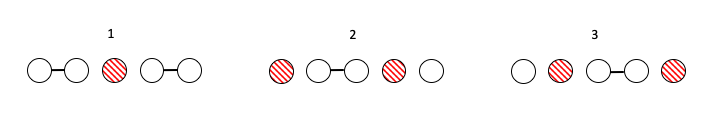
\includegraphics[width=\textwidth]{Figures/1d_CZschema.png}
\caption{$CZ$ schema for a $5$-qubit $1$D lattice. Here, we highlight in each layer the qubits excluded by the neighbouring $CZ$ restriction.}
\end{subfigure}
\begin{subfigure}[t]{0.85\textwidth}
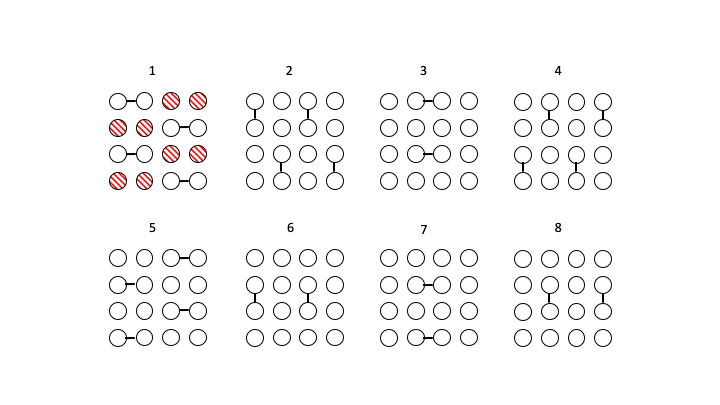
\includegraphics[width=\textwidth]{Figures/2D_CZschema.png}
\caption{$CZ$ schema for a $4\times 4$ qubit grid. As described in Algorithm~\ref{alg:cz_schema}, we apply $CZ$ gates along alternating the dimensions of the grid in each layer.}
\end{subfigure}
\begin{subfigure}[t]{0.8\textwidth}
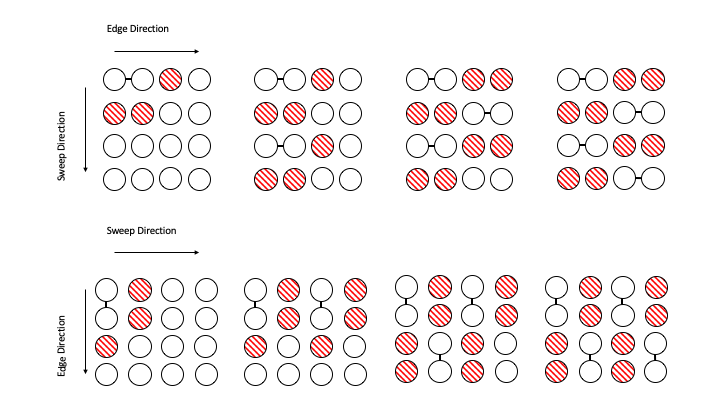
\includegraphics[width=\textwidth]{Figures/Algorithm_7_Example.png}
\caption{Example showing how two layers of $2$D schema are built up step-by-step using Algorithm~\ref{alg:cz_schema}, read left-to-right. Striped qubits indicated those excluded by the neighbouring $CZ$ restriction.}
\end{subfigure}
\end{figure}
Previous work has described two distinct rules for placing single-qubit gates. In the first scheme, we place one of the three gates with equal probability on any qubit that was acted on by a $CZ$ gate in the previous layer~\cite{Boixo2016}. However, with this strategy can produce configurations like $T\,CZ\,T$, which can be rearranged to cancel the $T$ gates as diagonal unitaries commute. Thus, an updated rule was proposed. The first single-qubit gate applied must always be a $T$ gate. Then, we apply either $\mathe^{-\mathi\frac{\pi}{4}X}$ or $\mathe^{-\mathi\frac{\pi}{4}Y}$ to qubits acted on by $CZ$ in the previous layer, and $T$ if a qubit was acted on by a one of these two rotations on the previous layer~\cite{Villalonga2018}. We use the second rule to place single-qubit gates, except in the $1$D case as otherwise this rule will never place more than a single $T$ gate on each qubit. An example random circuit for a $1$D lattice is shown in Figure~\ref{fig:random_1d_circ}.
\begin{figure}[H]
\centerline{
\Qcircuit @C=1em @R=.7em {
    \lstick{\ket{0}} & \gate{H} & \ctrl{1}\barrier[0.3em]{4} &\qw & \gate{T}\barrier[0.3em]{4}            &\qw & \qw & \qw \\
    \lstick{\ket{0}} & \gate{H} & \control \qw               &\qw & \ctrl{1}                              &\qw & \gate{\mathe^{-\mathi\frac{\pi}{4}Y}} & \qw \\
    \lstick{\ket{0}} & \gate{H} & \qw                        &\qw & \control \qw                          &\qw & \ctrl{1}      & \qw \\
    \lstick{\ket{0}} & \gate{H} & \ctrl{1}                   &\qw & \gate{\mathe^{-\mathi\frac{\pi}{4}X}} &\qw & \control \qw  & \qw \\
    \lstick{\ket{0}} & \gate{H} & \control \qw               &\qw & \gate{T}                              &\qw & \qw           & \qw\\
}}
\caption{Circuit diagram showing $3$ layers of the random circuit applied to a $5$-qubit, $1$D lattice. Each dashed line represents the end of a single layer.}\label{fig:random_1d_circ}
\end{figure}
We examined the performance and resource requirements of the stabilizer rank method for HOG, sampling $1000000$ amplitudes in the computational basis from the output distribution of Google circuits. We first consider how the runtime and requirements scale as a function of the circuit depth and the precision $\epsilon$, for a $4\times 5$ qubit grid, for $d\in [10, 20]$. We then pick a precision value $\epsilon=0.995$, comparable to that used in~\cite{Villalonga2018}, and explore how the runtime varies with depth for each connectivity pattern, for depth $d\in[15,25]$.\par
Circuits were generated using custom \texttt{C++} code, and interfaced with Python using \texttt{Pybind}. The resulting circuits were then convert to a \texttt{Qobj}, and run with our simulator as part of \texttt{Qiskit-Aer}. All simulations were run on UCL's Myriad computing cluster, with $2.3\mathrm{GHz}$ processors. The $4\times5$ qubit simulations were run with $36$ parallel workers and $32\mathrm{GB}$ of RAM.\ Due to scheduling restrictions on the cluster, the simulations for differing connectivities were run with $28$ parallel workers, and $28\mathrm{GB}$ of RAM.
\begin{figure}[H]
\centering
\caption{Resource Analysis of Google circuits on a $20$ qubit lattice.}\label{fig:rc_resources}
\begin{subfigure}[t]{0.48\textwidth}
\begin{scaletikzpicturetowidth}{\textwidth}
% This file was created by matplotlib2tikz v0.7.4.
\begin{tikzpicture}[scale=\tikzscale]

\definecolor{color0}{rgb}{0.12156862745098,0.466666666666667,0.705882352941177}
\definecolor{color1}{rgb}{0.83921568627451,0.152941176470588,0.156862745098039}
\definecolor{color2}{rgb}{0.580392156862745,0.403921568627451,0.741176470588235}
\definecolor{color3}{rgb}{0.549019607843137,0.337254901960784,0.294117647058824}
\definecolor{color4}{rgb}{1,0.498039215686275,0.0549019607843137}
\definecolor{color5}{rgb}{0.172549019607843,0.627450980392157,0.172549019607843}

\begin{axis}[
legend cell align={left},
legend style={at={(0.03,0.97)}, anchor=north west, draw=white!80.0!black},
tick align=outside,
tick pos=left,
x grid style={white!69.01960784313725!black},
xlabel={Depth},
xmin=3.5, xmax=36.5,
xtick style={color=black},
y grid style={white!69.01960784313725!black},
ylabel={T Count},
ymin=-2.8, ymax=146.8,
ytick style={color=black}
]
\path [draw=color0, semithick]
(axis cs:5,27)
--(axis cs:5,31);

\path [draw=color0, semithick]
(axis cs:6,29)
--(axis cs:6,33);

\path [draw=color0, semithick]
(axis cs:7,31)
--(axis cs:7,37);

\path [draw=color0, semithick]
(axis cs:8,34)
--(axis cs:8,40);

\path [draw=color0, semithick]
(axis cs:9,35)
--(axis cs:9,43);

\path [draw=color0, semithick]
(axis cs:10,38)
--(axis cs:10,46);

\path [draw=color0, semithick]
(axis cs:11,40)
--(axis cs:11,50);

\path [draw=color0, semithick]
(axis cs:12,43)
--(axis cs:12,53);

\path [draw=color0, semithick]
(axis cs:13,46)
--(axis cs:13,56);

\path [draw=color0, semithick]
(axis cs:14,48)
--(axis cs:14,60);

\path [draw=color0, semithick]
(axis cs:15,50)
--(axis cs:15,62);

\path [draw=color0, semithick]
(axis cs:16,52)
--(axis cs:16,64);

\path [draw=color0, semithick]
(axis cs:17,54)
--(axis cs:17,66);

\path [draw=color0, semithick]
(axis cs:18,57)
--(axis cs:18,69);

\path [draw=color0, semithick]
(axis cs:19,60)
--(axis cs:19,72);

\path [draw=color0, semithick]
(axis cs:20,62)
--(axis cs:20,74);

\path [draw=color0, semithick]
(axis cs:21,64)
--(axis cs:21,76);

\path [draw=color0, semithick]
(axis cs:22,66)
--(axis cs:22,80);

\path [draw=color0, semithick]
(axis cs:23,68)
--(axis cs:23,82);

\path [draw=color0, semithick]
(axis cs:24,70)
--(axis cs:24,86);

\path [draw=color0, semithick]
(axis cs:25,72)
--(axis cs:25,88);

\path [draw=color0, semithick]
(axis cs:26,75)
--(axis cs:26,91);

\path [draw=color0, semithick]
(axis cs:27,77)
--(axis cs:27,93);

\path [draw=color0, semithick]
(axis cs:28,78)
--(axis cs:28,96);

\path [draw=color0, semithick]
(axis cs:29,82)
--(axis cs:29,100);

\path [draw=color0, semithick]
(axis cs:30,85)
--(axis cs:30,101);

\path [draw=color0, semithick]
(axis cs:31,88)
--(axis cs:31,104);

\path [draw=color0, semithick]
(axis cs:32,90)
--(axis cs:32,108);

\path [draw=color0, semithick]
(axis cs:33,92)
--(axis cs:33,110);

\path [draw=color0, semithick]
(axis cs:34,95)
--(axis cs:34,113);

\path [draw=color0, semithick]
(axis cs:35,98)
--(axis cs:35,116);

\path [draw=color1, semithick]
(axis cs:5,5)
--(axis cs:5,5);

\path [draw=color1, semithick]
(axis cs:6,7)
--(axis cs:6,7);

\path [draw=color1, semithick]
(axis cs:7,9)
--(axis cs:7,9);

\path [draw=color1, semithick]
(axis cs:8,11)
--(axis cs:8,11);

\path [draw=color1, semithick]
(axis cs:9,12)
--(axis cs:9,12);

\path [draw=color1, semithick]
(axis cs:10,14)
--(axis cs:10,14);

\path [draw=color1, semithick]
(axis cs:11,16)
--(axis cs:11,16);

\path [draw=color1, semithick]
(axis cs:12,18)
--(axis cs:12,18);

\path [draw=color1, semithick]
(axis cs:13,19)
--(axis cs:13,21);

\path [draw=color1, semithick]
(axis cs:14,20)
--(axis cs:14,22);

\path [draw=color1, semithick]
(axis cs:15,23)
--(axis cs:15,23);

\path [draw=color1, semithick]
(axis cs:16,25)
--(axis cs:16,25);

\path [draw=color1, semithick]
(axis cs:17,26)
--(axis cs:17,28);

\path [draw=color1, semithick]
(axis cs:18,28)
--(axis cs:18,30);

\path [draw=color1, semithick]
(axis cs:19,30)
--(axis cs:19,32);

\path [draw=color1, semithick]
(axis cs:20,31)
--(axis cs:20,33);

\path [draw=color1, semithick]
(axis cs:21,33)
--(axis cs:21,35);

\path [draw=color1, semithick]
(axis cs:22,35)
--(axis cs:22,37);

\path [draw=color1, semithick]
(axis cs:23,37)
--(axis cs:23,39);

\path [draw=color1, semithick]
(axis cs:24,39)
--(axis cs:24,41);

\path [draw=color1, semithick]
(axis cs:25,40)
--(axis cs:25,42);

\path [draw=color1, semithick]
(axis cs:26,42)
--(axis cs:26,44);

\path [draw=color1, semithick]
(axis cs:27,44)
--(axis cs:27,46);

\path [draw=color1, semithick]
(axis cs:28,46)
--(axis cs:28,48);

\path [draw=color1, semithick]
(axis cs:29,48)
--(axis cs:29,50);

\path [draw=color1, semithick]
(axis cs:30,49)
--(axis cs:30,51);

\path [draw=color1, semithick]
(axis cs:31,51)
--(axis cs:31,53);

\path [draw=color1, semithick]
(axis cs:32,53)
--(axis cs:32,55);

\path [draw=color1, semithick]
(axis cs:33,55)
--(axis cs:33,57);

\path [draw=color1, semithick]
(axis cs:34,56)
--(axis cs:34,58);

\path [draw=color1, semithick]
(axis cs:35,58)
--(axis cs:35,60);

\path [draw=color2, semithick]
(axis cs:5,11)
--(axis cs:5,13);

\path [draw=color2, semithick]
(axis cs:6,15)
--(axis cs:6,17);

\path [draw=color2, semithick]
(axis cs:7,19)
--(axis cs:7,21);

\path [draw=color2, semithick]
(axis cs:8,22)
--(axis cs:8,26);

\path [draw=color2, semithick]
(axis cs:9,25)
--(axis cs:9,29);

\path [draw=color2, semithick]
(axis cs:10,29)
--(axis cs:10,33);

\path [draw=color2, semithick]
(axis cs:11,33)
--(axis cs:11,37);

\path [draw=color2, semithick]
(axis cs:12,37)
--(axis cs:12,41);

\path [draw=color2, semithick]
(axis cs:13,41)
--(axis cs:13,45);

\path [draw=color2, semithick]
(axis cs:14,44)
--(axis cs:14,50);

\path [draw=color2, semithick]
(axis cs:15,48)
--(axis cs:15,54);

\path [draw=color2, semithick]
(axis cs:16,52)
--(axis cs:16,58);

\path [draw=color2, semithick]
(axis cs:17,57)
--(axis cs:17,63);

\path [draw=color2, semithick]
(axis cs:18,60)
--(axis cs:18,66);

\path [draw=color2, semithick]
(axis cs:19,64)
--(axis cs:19,70);

\path [draw=color2, semithick]
(axis cs:20,68)
--(axis cs:20,74);

\path [draw=color2, semithick]
(axis cs:21,72)
--(axis cs:21,78);

\path [draw=color2, semithick]
(axis cs:22,76)
--(axis cs:22,82);

\path [draw=color2, semithick]
(axis cs:23,79)
--(axis cs:23,87);

\path [draw=color2, semithick]
(axis cs:24,83)
--(axis cs:24,91);

\path [draw=color2, semithick]
(axis cs:25,87)
--(axis cs:25,95);

\path [draw=color2, semithick]
(axis cs:26,91)
--(axis cs:26,99);

\path [draw=color2, semithick]
(axis cs:27,94)
--(axis cs:27,102);

\path [draw=color2, semithick]
(axis cs:28,98)
--(axis cs:28,106);

\path [draw=color2, semithick]
(axis cs:29,102)
--(axis cs:29,110);

\path [draw=color2, semithick]
(axis cs:30,106)
--(axis cs:30,114);

\path [draw=color2, semithick]
(axis cs:31,110)
--(axis cs:31,118);

\path [draw=color2, semithick]
(axis cs:32,113)
--(axis cs:32,121);

\path [draw=color2, semithick]
(axis cs:33,118)
--(axis cs:33,126);

\path [draw=color2, semithick]
(axis cs:34,121)
--(axis cs:34,129);

\path [draw=color2, semithick]
(axis cs:35,125)
--(axis cs:35,135);

\path [draw=color3, semithick]
(axis cs:5,4)
--(axis cs:5,6);

\path [draw=color3, semithick]
(axis cs:6,5)
--(axis cs:6,7);

\path [draw=color3, semithick]
(axis cs:7,7)
--(axis cs:7,9);

\path [draw=color3, semithick]
(axis cs:8,7)
--(axis cs:8,11);

\path [draw=color3, semithick]
(axis cs:9,9)
--(axis cs:9,13);

\path [draw=color3, semithick]
(axis cs:10,9)
--(axis cs:10,15);

\path [draw=color3, semithick]
(axis cs:11,11)
--(axis cs:11,17);

\path [draw=color3, semithick]
(axis cs:12,13)
--(axis cs:12,19);

\path [draw=color3, semithick]
(axis cs:13,15)
--(axis cs:13,21);

\path [draw=color3, semithick]
(axis cs:14,16)
--(axis cs:14,22);

\path [draw=color3, semithick]
(axis cs:15,18)
--(axis cs:15,24);

\path [draw=color3, semithick]
(axis cs:16,19)
--(axis cs:16,27);

\path [draw=color3, semithick]
(axis cs:17,22)
--(axis cs:17,28);

\path [draw=color3, semithick]
(axis cs:18,22)
--(axis cs:18,30);

\path [draw=color3, semithick]
(axis cs:19,23)
--(axis cs:19,31);

\path [draw=color3, semithick]
(axis cs:20,25)
--(axis cs:20,33);

\path [draw=color3, semithick]
(axis cs:21,27)
--(axis cs:21,35);

\path [draw=color3, semithick]
(axis cs:22,28)
--(axis cs:22,36);

\path [draw=color3, semithick]
(axis cs:23,30)
--(axis cs:23,38);

\path [draw=color3, semithick]
(axis cs:24,31)
--(axis cs:24,39);

\path [draw=color3, semithick]
(axis cs:25,33)
--(axis cs:25,41);

\path [draw=color3, semithick]
(axis cs:26,34)
--(axis cs:26,42);

\path [draw=color3, semithick]
(axis cs:27,36)
--(axis cs:27,44);

\path [draw=color3, semithick]
(axis cs:28,38)
--(axis cs:28,46);

\path [draw=color3, semithick]
(axis cs:29,39)
--(axis cs:29,47);

\path [draw=color3, semithick]
(axis cs:30,40)
--(axis cs:30,50);

\path [draw=color3, semithick]
(axis cs:31,42)
--(axis cs:31,52);

\path [draw=color3, semithick]
(axis cs:32,43)
--(axis cs:32,53);

\path [draw=color3, semithick]
(axis cs:33,45)
--(axis cs:33,55);

\path [draw=color3, semithick]
(axis cs:34,47)
--(axis cs:34,57);

\path [draw=color3, semithick]
(axis cs:35,48)
--(axis cs:35,60);

\addplot [semithick, color4]
table {%
5 14
6 18
7 24
8 30
9 32
10 34
11 38
12 47
13 48
14 52
15 58
16 64
17 66
18 68
19 72
20 81
21 82
22 86
23 92
24 98
25 100
26 102
27 106
28 115
29 116
30 120
31 126
32 132
33 134
34 136
35 140
};
\addlegendentry{2D Lattice}
\addplot [semithick, color5]
table {%
5 12
6 16
7 18
8 21
9 28
10 32
11 34
12 37
13 40
14 42
15 48
16 52
17 54
18 58
19 60
20 63
21 70
22 74
23 76
24 79
25 82
26 84
27 90
28 94
29 96
30 100
31 102
32 105
33 112
34 116
35 118
};
\addlegendentry{3D Lattice}
\addplot [semithick, black, dashed, forget plot]
table {%
168.5 100
1158.5 100
};
\addplot [semithick, color0]
table {%
5 29
6 31
7 34
8 37
9 39
10 42
11 45
12 48
13 51
14 54
15 56
16 58
17 60
18 63
19 66
20 68
21 70
22 73
23 75
24 78
25 80
26 83
27 85
28 87
29 91
30 93
31 96
32 99
33 101
34 104
35 107
};
\addlegendentry{$\infty, f=0.5$}
\addplot [semithick, color1]
table {%
5 5
6 7
7 9
8 11
9 12
10 14
11 16
12 18
13 20
14 21
15 23
16 25
17 27
18 29
19 31
20 32
21 34
22 36
23 38
24 40
25 41
26 43
27 45
28 47
29 49
30 50
31 52
32 54
33 56
34 57
35 59
};
\addlegendentry{$\infty, f=0.5$}
\addplot [semithick, color2]
table {%
5 12
6 16
7 20
8 24
9 27
10 31
11 35
12 39
13 43
14 47
15 51
16 55
17 60
18 63
19 67
20 71
21 75
22 79
23 83
24 87
25 91
26 95
27 98
28 102
29 106
30 110
31 114
32 117
33 122
34 125
35 130
};
\addlegendentry{$\infty, f=0.5$}
\addplot [semithick, color3]
table {%
5 5
6 6
7 8
8 9
9 11
10 12
11 14
12 16
13 18
14 19
15 21
16 23
17 25
18 26
19 27
20 29
21 31
22 32
23 34
24 35
25 37
26 38
27 40
28 42
29 43
30 45
31 47
32 48
33 50
34 52
35 54
};
\addlegendentry{$\infty, f=0.5$}
\end{axis}

\end{tikzpicture}
\end{scaletikzpicturetowidth}
\caption{Average $T$ count as a function of depth for a $24$ qubit lattice with different connectivity patterns.}\label{fig:t_count_depth}
\end{subfigure}
\begin{subfigure}[t]{0.48\textwidth}
\begin{scaletikzpicturetowidth}{\textwidth}
% This file was created by matplotlib2tikz v0.7.4.
\begin{tikzpicture}[scale=\tikzscale]

\definecolor{color0}{rgb}{0.12156862745098,0.466666666666667,0.705882352941177}
\definecolor{color1}{rgb}{1,0.498039215686275,0.0549019607843137}
\definecolor{color2}{rgb}{0.172549019607843,0.627450980392157,0.172549019607843}

\begin{axis}[
legend cell align={left},
legend style={at={(0.03,0.97)}, anchor=north west, draw=white!80.0!black},
tick align=outside,
tick pos=left,
x grid style={white!69.01960784313725!black},
xlabel={Depth},
xmin=3.5, xmax=36.5,
xtick style={color=black},
y grid style={white!69.01960784313725!black},
ylabel={T Count},
ymin=0.75, ymax=248.25,
ytick style={color=black}
]
\addplot [semithick, color0]
table {%
5 12
6 15
7 20
8 26
9 27
10 30
11 34
12 40
13 42
14 45
15 50
16 56
17 57
18 60
19 64
20 70
21 72
22 75
23 80
24 86
25 87
26 90
27 94
28 100
29 102
30 105
31 110
32 116
33 117
34 120
35 124
};
\addlegendentry{$4\times 5$ Lattice}
\addplot [semithick, color1]
table {%
5 14
6 18
7 24
8 30
9 32
10 34
11 38
12 47
13 48
14 52
15 58
16 64
17 66
18 68
19 72
20 81
21 82
22 86
23 92
24 98
25 100
26 102
27 106
28 115
29 116
30 120
31 126
32 132
33 134
34 136
35 140
};
\addlegendentry{$4\times 6$ Lattice}
\addplot [semithick, color2]
table {%
5 25
6 33
7 41
8 49
9 53
10 57
11 66
12 75
13 82
14 90
15 98
16 106
17 110
18 114
19 123
20 132
21 139
22 147
23 155
24 163
25 167
26 171
27 180
28 189
29 196
30 204
31 212
32 220
33 224
34 228
35 237
};
\addlegendentry{$6\times 6$ Lattice}
\end{axis}

\end{tikzpicture}
\end{scaletikzpicturetowidth}
\caption{$T$ count as a function of depth for different sizes of $2$D qubit lattices.}\label{fig:t_count_connectivity}
\end{subfigure}
\begin{subfigure}[t]{0.48\textwidth}
\begin{scaletikzpicturetowidth}{\textwidth}
% This file was created by matplotlib2tikz v0.7.4.
\begin{tikzpicture}[scale=\tikzscale]

\definecolor{color0}{rgb}{0.12156862745098,0.466666666666667,0.705882352941177}
\definecolor{color1}{rgb}{1,0.498039215686275,0.0549019607843137}
\definecolor{color2}{rgb}{0.172549019607843,0.627450980392157,0.172549019607843}
\definecolor{color3}{rgb}{0.83921568627451,0.152941176470588,0.156862745098039}

\begin{axis}[
legend cell align={left},
legend style={at={(0.03,0.07)}, anchor=south west, draw=white!80.0!black},
tick align=outside,
tick pos=left,
x grid style={white!69.01960784313725!black},
xlabel={Approximation Error},
xmin=-0.69, xmax=5.69,
xtick style={color=black},
xtick={-1,0,1,2,3,4,5,6},
xticklabels={,0.1,0.5,0.75,0.9,0.99,0.995,},
y grid style={white!69.01960784313725!black},
ylabel={Maximum T Count},
ymin=0, ymax=127.05,
ytick style={color=black}
]
\draw[fill=color0,draw opacity=0] (axis cs:-0.4,0) rectangle (axis cs:-0.2,92);
\addlegendimage{ybar,ybar legend,fill=color0,draw opacity=0};
\addlegendentry{20 qubits}

\draw[fill=color0,draw opacity=0] (axis cs:0.6,0) rectangle (axis cs:0.8,112);
\draw[fill=color0,draw opacity=0] (axis cs:1.6,0) rectangle (axis cs:1.8,117);
\draw[fill=color0,draw opacity=0] (axis cs:2.6,0) rectangle (axis cs:2.8,120);
\draw[fill=color0,draw opacity=0] (axis cs:3.6,0) rectangle (axis cs:3.8,121);
\draw[fill=color0,draw opacity=0] (axis cs:4.6,0) rectangle (axis cs:4.8,121);
\draw[fill=color1,draw opacity=0] (axis cs:-0.2,0) rectangle (axis cs:0,89);
\addlegendimage{ybar,ybar legend,fill=color1,draw opacity=0};
\addlegendentry{30 qubits}

\draw[fill=color1,draw opacity=0] (axis cs:0.8,0) rectangle (axis cs:1,110);
\draw[fill=color1,draw opacity=0] (axis cs:1.8,0) rectangle (axis cs:2,115);
\draw[fill=color1,draw opacity=0] (axis cs:2.8,0) rectangle (axis cs:3,117);
\draw[fill=color1,draw opacity=0] (axis cs:3.8,0) rectangle (axis cs:4,118);
\draw[fill=color1,draw opacity=0] (axis cs:4.8,0) rectangle (axis cs:5,118);
\draw[fill=color2,draw opacity=0] (axis cs:-1.38777878078145e-17,0) rectangle (axis cs:0.2,88);
\addlegendimage{ybar,ybar legend,fill=color2,draw opacity=0};
\addlegendentry{40 qubits}

\draw[fill=color2,draw opacity=0] (axis cs:1,0) rectangle (axis cs:1.2,108);
\draw[fill=color2,draw opacity=0] (axis cs:2,0) rectangle (axis cs:2.2,113);
\draw[fill=color2,draw opacity=0] (axis cs:3,0) rectangle (axis cs:3.2,115);
\draw[fill=color2,draw opacity=0] (axis cs:4,0) rectangle (axis cs:4.2,117);
\draw[fill=color2,draw opacity=0] (axis cs:5,0) rectangle (axis cs:5.2,117);
\draw[fill=color3,draw opacity=0] (axis cs:0.2,0) rectangle (axis cs:0.4,86);
\addlegendimage{ybar,ybar legend,fill=color3,draw opacity=0};
\addlegendentry{50 qubits}

\draw[fill=color3,draw opacity=0] (axis cs:1.2,0) rectangle (axis cs:1.4,107);
\draw[fill=color3,draw opacity=0] (axis cs:2.2,0) rectangle (axis cs:2.4,112);
\draw[fill=color3,draw opacity=0] (axis cs:3.2,0) rectangle (axis cs:3.4,114);
\draw[fill=color3,draw opacity=0] (axis cs:4.2,0) rectangle (axis cs:4.4,115);
\draw[fill=color3,draw opacity=0] (axis cs:5.2,0) rectangle (axis cs:5.4,115);
\end{axis}

\end{tikzpicture}
\end{scaletikzpicturetowidth}
\caption{Plot showing the maximum number of $T$ gates that can be simulated for different system sizes, assuming access to $192\mathrm{GB}$ of RAM.}\label{fig:max_t_bar}
\end{subfigure}
\begin{subfigure}[t]{0.48\textwidth}
\begin{scaletikzpicturetowidth}{\textwidth}
% This file was created by matplotlib2tikz v0.7.4.
\begin{tikzpicture}[scale=\tikzscale]

\definecolor{color0}{rgb}{0.12156862745098,0.466666666666667,0.705882352941177}
\definecolor{color1}{rgb}{1,0.498039215686275,0.0549019607843137}
\definecolor{color2}{rgb}{0.172549019607843,0.627450980392157,0.172549019607843}
\definecolor{color3}{rgb}{0.83921568627451,0.152941176470588,0.156862745098039}

\begin{axis}[
legend cell align={left},
legend style={at={(0.03,0.97)}, anchor=north west, draw=white!80.0!black},
tick align=outside,
tick pos=left,
x grid style={white!69.01960784313725!black},
xlabel={Approximation Error},
xmin=-0.69, xmax=5.69,
xtick style={color=black},
xtick={-1,0,1,2,3,4,5,6},
xticklabels={,0.1,0.5,0.75,0.9,0.99,0.995,},
y grid style={white!69.01960784313725!black},
ylabel={Maximum Extent (\(\displaystyle 192\mathrm{GB}\))},
ymin=0, ymax=204379176.96,
ytick style={color=black}
]
\draw[fill=color0,draw opacity=0] (axis cs:-0.4,0) rectangle (axis cs:-0.2,1966080);
\addlegendimage{ybar,ybar legend,fill=color0,draw opacity=0};
\addlegendentry{20 qubits}

\draw[fill=color0,draw opacity=0] (axis cs:0.6,0) rectangle (axis cs:0.8,49152000);
\draw[fill=color0,draw opacity=0] (axis cs:1.6,0) rectangle (axis cs:1.8,110592000);
\draw[fill=color0,draw opacity=0] (axis cs:2.6,0) rectangle (axis cs:2.8,159252480);
\draw[fill=color0,draw opacity=0] (axis cs:3.6,0) rectangle (axis cs:3.8,192695500.8);
\draw[fill=color0,draw opacity=0] (axis cs:4.6,0) rectangle (axis cs:4.8,194646835.2);
\draw[fill=color1,draw opacity=0] (axis cs:-0.2,0) rectangle (axis cs:0,1310720);
\addlegendimage{ybar,ybar legend,fill=color1,draw opacity=0};
\addlegendentry{30 qubits}

\draw[fill=color1,draw opacity=0] (axis cs:0.8,0) rectangle (axis cs:1,32768000);
\draw[fill=color1,draw opacity=0] (axis cs:1.8,0) rectangle (axis cs:2,73728000);
\draw[fill=color1,draw opacity=0] (axis cs:2.8,0) rectangle (axis cs:3,106168320);
\draw[fill=color1,draw opacity=0] (axis cs:3.8,0) rectangle (axis cs:4,128463667.2);
\draw[fill=color1,draw opacity=0] (axis cs:4.8,0) rectangle (axis cs:5,129764556.8);
\draw[fill=color2,draw opacity=0] (axis cs:-1.38777878078145e-17,0) rectangle (axis cs:0.2,983040);
\addlegendimage{ybar,ybar legend,fill=color2,draw opacity=0};
\addlegendentry{40 qubits}

\draw[fill=color2,draw opacity=0] (axis cs:1,0) rectangle (axis cs:1.2,24576000);
\draw[fill=color2,draw opacity=0] (axis cs:2,0) rectangle (axis cs:2.2,55296000);
\draw[fill=color2,draw opacity=0] (axis cs:3,0) rectangle (axis cs:3.2,79626240);
\draw[fill=color2,draw opacity=0] (axis cs:4,0) rectangle (axis cs:4.2,96347750.4);
\draw[fill=color2,draw opacity=0] (axis cs:5,0) rectangle (axis cs:5.2,97323417.6);
\draw[fill=color3,draw opacity=0] (axis cs:0.2,0) rectangle (axis cs:0.4,786432);
\addlegendimage{ybar,ybar legend,fill=color3,draw opacity=0};
\addlegendentry{50 qubits}

\draw[fill=color3,draw opacity=0] (axis cs:1.2,0) rectangle (axis cs:1.4,19660800);
\draw[fill=color3,draw opacity=0] (axis cs:2.2,0) rectangle (axis cs:2.4,44236800);
\draw[fill=color3,draw opacity=0] (axis cs:3.2,0) rectangle (axis cs:3.4,63700992);
\draw[fill=color3,draw opacity=0] (axis cs:4.2,0) rectangle (axis cs:4.4,77078200.32);
\draw[fill=color3,draw opacity=0] (axis cs:5.2,0) rectangle (axis cs:5.4,77858734.08);
\end{axis}

\end{tikzpicture}
\end{scaletikzpicturetowidth}
\caption{Plot showing the maximum circuit extent that can be simulated for different system sizes, assuming access to $192\mathrm{GB}$ of RAM.}\label{fig:max_extent_bar}
\end{subfigure}
\end{figure}
\begin{figure}[t]
\centering
\begin{scaletikzpicturetowidth}{0.75\textwidth}
% This file was created by matplotlib2tikz v0.7.4.
\begin{tikzpicture}[scale=\tikzscale]

\definecolor{color0}{rgb}{0.12156862745098,0.466666666666667,0.705882352941177}
\definecolor{color1}{rgb}{1,0.498039215686275,0.0549019607843137}
\definecolor{color2}{rgb}{0.172549019607843,0.627450980392157,0.172549019607843}
\definecolor{color3}{rgb}{0.83921568627451,0.152941176470588,0.156862745098039}
\definecolor{color4}{rgb}{0.580392156862745,0.403921568627451,0.741176470588235}
\definecolor{color5}{rgb}{0.549019607843137,0.337254901960784,0.294117647058824}

\begin{axis}[
legend cell align={left},
legend style={at={(0.03,0.97)}, anchor=north west, draw=white!80.0!black},
tick align=outside,
tick pos=left,
x grid style={white!69.01960784313725!black},
xlabel={Depth},
xmin=-0.5, xmax=10.5,
xtick style={color=black},
xtick={0,1,2,3,4,5,6,7,8,9,10},
xtick={0,1,2,3,4,5,6,7,8,9,10},
xtick={0,1,2,3,4,5,6,7,8,9,10},
xtick={0,1,2,3,4,5,6,7,8,9,10},
xtick={0,1,2,3,4,5,6,7,8,9,10},
xtick={0,1,2,3,4,5,6,7,8,9,10},
xticklabels={10,11,12,13,14,15,16,17,18,19,20},
xticklabels={10,11,12,13,14,15,16,17,18,19,20},
xticklabels={10,11,12,13,14,15,16,17,18,19,20},
xticklabels={10,11,12,13,14,15,16,17,18,19,20},
xticklabels={10,11,12,13,14,15,16,17,18,19,20},
xticklabels={10,11,12,13,14,15,16,17,18,19,20},
y grid style={white!69.01960784313725!black},
ylabel={\(\displaystyle \log\left(\text{Runtime}\right) / \mathrm{s}\)},
ymin=0.21626108403158, ymax=3.9158141504768,
ytick style={color=black}
]
\path [draw=color0, semithick]
(axis cs:0,0.576774912857408)
--(axis cs:0,0.619736615186687);

\path [draw=color0, semithick]
(axis cs:1,0.656395715094232)
--(axis cs:1,0.785591944804676);

\path [draw=color0, semithick]
(axis cs:2,1.2391668696604)
--(axis cs:2,1.33758366218233);

\path [draw=color0, semithick]
(axis cs:3,1.32143322199428)
--(axis cs:3,1.37728503796167);

\path [draw=color0, semithick]
(axis cs:4,1.67268360788086)
--(axis cs:4,1.70616127836048);

\path [draw=color0, semithick]
(axis cs:5,1.99639960725369)
--(axis cs:5,2.02889298935853);

\path [draw=color0, semithick]
(axis cs:6,2.44557694824556)
--(axis cs:6,2.48908980087762);

\path [draw=color0, semithick]
(axis cs:7,2.44486071229482)
--(axis cs:7,2.47970603625271);

\path [draw=color0, semithick]
(axis cs:8,2.71444668831868)
--(axis cs:8,2.74817773947729);

\path [draw=color0, semithick]
(axis cs:9,2.98553134023438)
--(axis cs:9,3.03350617891376);

\path [draw=color0, semithick]
(axis cs:10,3.71467616928272)
--(axis cs:10,3.74765264745657);

\path [draw=color1, semithick]
(axis cs:0,0.442873314980508)
--(axis cs:0,0.478047248512298);

\path [draw=color1, semithick]
(axis cs:1,0.479119941202655)
--(axis cs:1,0.513324191768444);

\path [draw=color1, semithick]
(axis cs:2,0.571604779740352)
--(axis cs:2,0.679485322769323);

\path [draw=color1, semithick]
(axis cs:3,0.602802142657569)
--(axis cs:3,0.717350369737927);

\path [draw=color1, semithick]
(axis cs:4,0.88893097059032)
--(axis cs:4,0.946755380760654);

\path [draw=color1, semithick]
(axis cs:5,1.28141042544491)
--(axis cs:5,1.34366234403035);

\path [draw=color1, semithick]
(axis cs:6,1.80100029097524)
--(axis cs:6,1.86169073169443);

\path [draw=color1, semithick]
(axis cs:7,1.81582040410373)
--(axis cs:7,1.84732752969695);

\path [draw=color1, semithick]
(axis cs:8,2.10267427679897)
--(axis cs:8,2.13476041508467);

\path [draw=color1, semithick]
(axis cs:9,2.36117303719268)
--(axis cs:9,2.43388945015034);

\path [draw=color1, semithick]
(axis cs:10,3.09322063046383)
--(axis cs:10,3.16246556399485);

\path [draw=color2, semithick]
(axis cs:0,0.546287616109396)
--(axis cs:0,0.57753747846679);

\path [draw=color2, semithick]
(axis cs:1,0.530698514771216)
--(axis cs:1,0.604834650625307);

\path [draw=color2, semithick]
(axis cs:2,0.494137447776922)
--(axis cs:2,0.544709730295193);

\path [draw=color2, semithick]
(axis cs:3,0.501236885398763)
--(axis cs:3,0.548636007494856);

\path [draw=color2, semithick]
(axis cs:4,0.577461382276083)
--(axis cs:4,0.687503685625991);

\path [draw=color2, semithick]
(axis cs:5,0.798197277825489)
--(axis cs:5,0.862201719263455);

\path [draw=color2, semithick]
(axis cs:6,1.37659011081827)
--(axis cs:6,1.42427408072307);

\path [draw=color2, semithick]
(axis cs:7,1.38274951618851)
--(axis cs:7,1.4245256451197);

\path [draw=color2, semithick]
(axis cs:8,1.69127747539748)
--(axis cs:8,1.74593203669655);

\path [draw=color2, semithick]
(axis cs:9,1.9843948359101)
--(axis cs:9,2.055459381641);

\path [draw=color2, semithick]
(axis cs:10,2.71277828480783)
--(axis cs:10,2.86176260852331);

\path [draw=color3, semithick]
(axis cs:0,0.538880801631908)
--(axis cs:0,0.583470512250956);

\path [draw=color3, semithick]
(axis cs:1,0.52789869325872)
--(axis cs:1,0.603857936041078);

\path [draw=color3, semithick]
(axis cs:2,0.453522644781292)
--(axis cs:2,0.498416399480816);

\path [draw=color3, semithick]
(axis cs:3,0.476963863837793)
--(axis cs:3,0.505082376949152);

\path [draw=color3, semithick]
(axis cs:4,0.513133491332384)
--(axis cs:4,0.589673016916064);

\path [draw=color3, semithick]
(axis cs:5,0.675604999693674)
--(axis cs:5,0.720716328585432);

\path [draw=color3, semithick]
(axis cs:6,1.1615752137297)
--(axis cs:6,1.21578023954806);

\path [draw=color3, semithick]
(axis cs:7,1.12983902387804)
--(axis cs:7,1.25924431080724);

\path [draw=color3, semithick]
(axis cs:8,1.51773095208035)
--(axis cs:8,1.54968464493542);

\path [draw=color3, semithick]
(axis cs:9,1.82460768711241)
--(axis cs:9,1.90271497910507);

\path [draw=color3, semithick]
(axis cs:10,2.53582238398843)
--(axis cs:10,2.6729819787069);

\path [draw=color4, semithick]
(axis cs:0,0.537754991538001)
--(axis cs:0,0.59004100076719);

\path [draw=color4, semithick]
(axis cs:1,0.538780025528615)
--(axis cs:1,0.597554677947111);

\path [draw=color4, semithick]
(axis cs:2,0.384422587051817)
--(axis cs:2,0.590047949432477);

\path [draw=color4, semithick]
(axis cs:3,0.460345448275061)
--(axis cs:3,0.503984521928215);

\path [draw=color4, semithick]
(axis cs:4,0.512670278306361)
--(axis cs:4,0.557627186067406);

\path [draw=color4, semithick]
(axis cs:5,0.631966877364537)
--(axis cs:5,0.696088978869495);

\path [draw=color4, semithick]
(axis cs:6,1.05588160342954)
--(axis cs:6,1.09975299840082);

\path [draw=color4, semithick]
(axis cs:7,1.05175132563624)
--(axis cs:7,1.1022259978191);

\path [draw=color4, semithick]
(axis cs:8,1.39415379388674)
--(axis cs:8,1.4553561055992);

\path [draw=color4, semithick]
(axis cs:9,1.74138374639561)
--(axis cs:9,1.80796815237723);

\path [draw=color4, semithick]
(axis cs:10,2.49223077380021)
--(axis cs:10,2.60412798648254);

\path [draw=color5, semithick]
(axis cs:0,0.549474181635389)
--(axis cs:0,0.578755355454212);

\path [draw=color5, semithick]
(axis cs:1,0.561568126934359)
--(axis cs:1,0.592395250446191);

\path [draw=color5, semithick]
(axis cs:2,0.408564661876319)
--(axis cs:2,0.564043999968559);

\path [draw=color5, semithick]
(axis cs:3,0.453512317535922)
--(axis cs:3,0.483040261021531);

\path [draw=color5, semithick]
(axis cs:4,0.493047964118473)
--(axis cs:4,0.561909530316726);

\path [draw=color5, semithick]
(axis cs:5,0.61626747374628)
--(axis cs:5,0.686576362227718);

\path [draw=color5, semithick]
(axis cs:6,1.01456205087355)
--(axis cs:6,1.13529092355614);

\path [draw=color5, semithick]
(axis cs:7,1.0393891016675)
--(axis cs:7,1.12224817640412);

\path [draw=color5, semithick]
(axis cs:8,1.3818427483935)
--(axis cs:8,1.48261707222237);

\path [draw=color5, semithick]
(axis cs:9,1.69355340900777)
--(axis cs:9,1.8517806200088);

\path [draw=color5, semithick]
(axis cs:10,2.46686385121206)
--(axis cs:10,2.61929417793009);

\addplot [semithick, color0]
table {%
0 0.598255764022047
1 0.720993829949454
2 1.28837526592136
3 1.34935912997798
4 1.68942244312067
5 2.01264629830611
6 2.46733337456159
7 2.46228337427377
8 2.73131221389799
9 3.00951875957407
10 3.73116440836964
};
\addlegendentry{$\epsilon=0.25$}
\addplot [semithick, color1]
table {%
0 0.460460281746403
1 0.496222066485549
2 0.625545051254838
3 0.660076256197748
4 0.917843175675487
5 1.31253638473763
6 1.83134551133483
7 1.83157396690034
8 2.11871734594182
9 2.39753124367151
10 3.12784309722934
};
\addlegendentry{$\epsilon=0.5$}
\addplot [semithick, color2]
table {%
0 0.561912547288093
1 0.567766582698262
2 0.519423589036058
3 0.524936446446809
4 0.632482533951037
5 0.830199498544472
6 1.40043209577067
7 1.40363758065411
8 1.71860475604702
9 2.01992710877555
10 2.78727044666557
};
\addlegendentry{$\epsilon=0.75$}
\addplot [semithick, color3]
table {%
0 0.561175656941432
1 0.565878314649899
2 0.475969522131054
3 0.491023120393472
4 0.551403254124224
5 0.698160664139553
6 1.18867772663888
7 1.19454166734264
8 1.53370779850789
9 1.86366133310874
10 2.60440218134766
};
\addlegendentry{$\epsilon=0.9$}
\addplot [semithick, color4]
table {%
0 0.563897996152596
1 0.568167351737863
2 0.487235268242147
3 0.482164985101638
4 0.535148732186884
5 0.664027928117016
6 1.07781730091518
7 1.07698866172767
8 1.42475494974297
9 1.77467594938642
10 2.54817938014138
};
\addlegendentry{$\epsilon=0.99$}
\addplot [semithick, color5]
table {%
0 0.564114768544801
1 0.576981688690275
2 0.486304330922439
3 0.468276289278726
4 0.5274787472176
5 0.651421917986999
6 1.07492648721484
7 1.08081863903581
8 1.43222991030793
9 1.77266701450828
10 2.54307901457107
};
\addlegendentry{$\epsilon=0.995$}
\end{axis}

\begin{axis}[
axis y line=right,
legend cell align={left},
legend style={at={(0.97,0.03)}, anchor=south east, draw=white!80.0!black},
tick align=outside,
x grid style={white!69.01960784313725!black},
xmin=-0.5, xmax=10.5,
xtick pos=left,
xtick style={color=black},
xtick={0,1,2,3,4,5,6,7,8,9,10},
xticklabels={10,11,12,13,14,15,16,17,18,19,20},
y grid style={white!69.01960784313725!black},
ylabel={T Count},
ymin=26.15, ymax=66.85,
ytick pos=right,
ytick style={color=black}
]
\addplot [semithick, black, dashed]
table {%
0 28
1 31
2 37
3 38
4 42
5 46
6 52
7 52
8 56
9 59
10 65
};
\addlegendentry{T Count}
\end{axis}

\end{tikzpicture}
\end{scaletikzpicturetowidth}
\caption{Average time required in seconds to take $1000000$ samples from the output distribution of a Google circuit, for different values of the precision $\epsilon$. Also shown is the corresponding $T$ count of the circuit.}\label{fig:precision_runtimes}
\end{figure}
\begin{figure}[t]
\centering
% \begin{scaletikzpicturetowidth}{0.75\textwidth}
% % This file was created by matplotlib2tikz v0.7.4.
\begin{tikzpicture}[scale=\tikzscale]

\definecolor{color0}{rgb}{0.12156862745098,0.466666666666667,0.705882352941177}
\definecolor{color1}{rgb}{1,0.498039215686275,0.0549019607843137}
\definecolor{color2}{rgb}{0.172549019607843,0.627450980392157,0.172549019607843}
\definecolor{color3}{rgb}{0.83921568627451,0.152941176470588,0.156862745098039}
\definecolor{color4}{rgb}{0.580392156862745,0.403921568627451,0.741176470588235}
\definecolor{color5}{rgb}{0.549019607843137,0.337254901960784,0.294117647058824}

\begin{axis}[
legend cell align={left},
legend style={at={(0.03,0.97)}, anchor=north west, draw=white!80.0!black},
tick align=outside,
tick pos=left,
x grid style={white!69.01960784313725!black},
xlabel={Depth},
xmin=-0.5, xmax=10.5,
xtick style={color=black},
xtick={0,1,2,3,4,5,6,7,8,9,10},
xtick={0,1,2,3,4,5,6,7,8,9,10},
xtick={0,1,2,3,4,5,6,7,8,9,10},
xtick={0,1,2,3,4,5,6,7,8,9,10},
xtick={0,1,2,3,4,5,6,7,8,9,10},
xtick={0,1,2,3,4,5,6,7,8,9,10},
xticklabels={10,11,12,13,14,15,16,17,18,19,20},
xticklabels={10,11,12,13,14,15,16,17,18,19,20},
xticklabels={10,11,12,13,14,15,16,17,18,19,20},
xticklabels={10,11,12,13,14,15,16,17,18,19,20},
xticklabels={10,11,12,13,14,15,16,17,18,19,20},
xticklabels={10,11,12,13,14,15,16,17,18,19,20},
y grid style={white!69.01960784313725!black},
ylabel={\(\displaystyle \log\left(\text{Runtime}\right) / \mathrm{s}\)},
ymin=0.21626108403158, ymax=3.9158141504768,
ytick style={color=black}
]
\path [draw=color0, semithick]
(axis cs:0,0.576774912857408)
--(axis cs:0,0.619736615186687);

\path [draw=color0, semithick]
(axis cs:1,0.656395715094232)
--(axis cs:1,0.785591944804676);

\path [draw=color0, semithick]
(axis cs:2,1.2391668696604)
--(axis cs:2,1.33758366218233);

\path [draw=color0, semithick]
(axis cs:3,1.32143322199428)
--(axis cs:3,1.37728503796167);

\path [draw=color0, semithick]
(axis cs:4,1.67268360788086)
--(axis cs:4,1.70616127836048);

\path [draw=color0, semithick]
(axis cs:5,1.99639960725369)
--(axis cs:5,2.02889298935853);

\path [draw=color0, semithick]
(axis cs:6,2.44557694824556)
--(axis cs:6,2.48908980087762);

\path [draw=color0, semithick]
(axis cs:7,2.44486071229482)
--(axis cs:7,2.47970603625271);

\path [draw=color0, semithick]
(axis cs:8,2.71444668831868)
--(axis cs:8,2.74817773947729);

\path [draw=color0, semithick]
(axis cs:9,2.98553134023438)
--(axis cs:9,3.03350617891376);

\path [draw=color0, semithick]
(axis cs:10,3.71467616928272)
--(axis cs:10,3.74765264745657);

\path [draw=color1, semithick]
(axis cs:0,0.442873314980508)
--(axis cs:0,0.478047248512298);

\path [draw=color1, semithick]
(axis cs:1,0.479119941202655)
--(axis cs:1,0.513324191768444);

\path [draw=color1, semithick]
(axis cs:2,0.571604779740352)
--(axis cs:2,0.679485322769323);

\path [draw=color1, semithick]
(axis cs:3,0.602802142657569)
--(axis cs:3,0.717350369737927);

\path [draw=color1, semithick]
(axis cs:4,0.88893097059032)
--(axis cs:4,0.946755380760654);

\path [draw=color1, semithick]
(axis cs:5,1.28141042544491)
--(axis cs:5,1.34366234403035);

\path [draw=color1, semithick]
(axis cs:6,1.80100029097524)
--(axis cs:6,1.86169073169443);

\path [draw=color1, semithick]
(axis cs:7,1.81582040410373)
--(axis cs:7,1.84732752969695);

\path [draw=color1, semithick]
(axis cs:8,2.10267427679897)
--(axis cs:8,2.13476041508467);

\path [draw=color1, semithick]
(axis cs:9,2.36117303719268)
--(axis cs:9,2.43388945015034);

\path [draw=color1, semithick]
(axis cs:10,3.09322063046383)
--(axis cs:10,3.16246556399485);

\path [draw=color2, semithick]
(axis cs:0,0.546287616109396)
--(axis cs:0,0.57753747846679);

\path [draw=color2, semithick]
(axis cs:1,0.530698514771216)
--(axis cs:1,0.604834650625307);

\path [draw=color2, semithick]
(axis cs:2,0.494137447776922)
--(axis cs:2,0.544709730295193);

\path [draw=color2, semithick]
(axis cs:3,0.501236885398763)
--(axis cs:3,0.548636007494856);

\path [draw=color2, semithick]
(axis cs:4,0.577461382276083)
--(axis cs:4,0.687503685625991);

\path [draw=color2, semithick]
(axis cs:5,0.798197277825489)
--(axis cs:5,0.862201719263455);

\path [draw=color2, semithick]
(axis cs:6,1.37659011081827)
--(axis cs:6,1.42427408072307);

\path [draw=color2, semithick]
(axis cs:7,1.38274951618851)
--(axis cs:7,1.4245256451197);

\path [draw=color2, semithick]
(axis cs:8,1.69127747539748)
--(axis cs:8,1.74593203669655);

\path [draw=color2, semithick]
(axis cs:9,1.9843948359101)
--(axis cs:9,2.055459381641);

\path [draw=color2, semithick]
(axis cs:10,2.71277828480783)
--(axis cs:10,2.86176260852331);

\path [draw=color3, semithick]
(axis cs:0,0.538880801631908)
--(axis cs:0,0.583470512250956);

\path [draw=color3, semithick]
(axis cs:1,0.52789869325872)
--(axis cs:1,0.603857936041078);

\path [draw=color3, semithick]
(axis cs:2,0.453522644781292)
--(axis cs:2,0.498416399480816);

\path [draw=color3, semithick]
(axis cs:3,0.476963863837793)
--(axis cs:3,0.505082376949152);

\path [draw=color3, semithick]
(axis cs:4,0.513133491332384)
--(axis cs:4,0.589673016916064);

\path [draw=color3, semithick]
(axis cs:5,0.675604999693674)
--(axis cs:5,0.720716328585432);

\path [draw=color3, semithick]
(axis cs:6,1.1615752137297)
--(axis cs:6,1.21578023954806);

\path [draw=color3, semithick]
(axis cs:7,1.12983902387804)
--(axis cs:7,1.25924431080724);

\path [draw=color3, semithick]
(axis cs:8,1.51773095208035)
--(axis cs:8,1.54968464493542);

\path [draw=color3, semithick]
(axis cs:9,1.82460768711241)
--(axis cs:9,1.90271497910507);

\path [draw=color3, semithick]
(axis cs:10,2.53582238398843)
--(axis cs:10,2.6729819787069);

\path [draw=color4, semithick]
(axis cs:0,0.537754991538001)
--(axis cs:0,0.59004100076719);

\path [draw=color4, semithick]
(axis cs:1,0.538780025528615)
--(axis cs:1,0.597554677947111);

\path [draw=color4, semithick]
(axis cs:2,0.384422587051817)
--(axis cs:2,0.590047949432477);

\path [draw=color4, semithick]
(axis cs:3,0.460345448275061)
--(axis cs:3,0.503984521928215);

\path [draw=color4, semithick]
(axis cs:4,0.512670278306361)
--(axis cs:4,0.557627186067406);

\path [draw=color4, semithick]
(axis cs:5,0.631966877364537)
--(axis cs:5,0.696088978869495);

\path [draw=color4, semithick]
(axis cs:6,1.05588160342954)
--(axis cs:6,1.09975299840082);

\path [draw=color4, semithick]
(axis cs:7,1.05175132563624)
--(axis cs:7,1.1022259978191);

\path [draw=color4, semithick]
(axis cs:8,1.39415379388674)
--(axis cs:8,1.4553561055992);

\path [draw=color4, semithick]
(axis cs:9,1.74138374639561)
--(axis cs:9,1.80796815237723);

\path [draw=color4, semithick]
(axis cs:10,2.49223077380021)
--(axis cs:10,2.60412798648254);

\path [draw=color5, semithick]
(axis cs:0,0.549474181635389)
--(axis cs:0,0.578755355454212);

\path [draw=color5, semithick]
(axis cs:1,0.561568126934359)
--(axis cs:1,0.592395250446191);

\path [draw=color5, semithick]
(axis cs:2,0.408564661876319)
--(axis cs:2,0.564043999968559);

\path [draw=color5, semithick]
(axis cs:3,0.453512317535922)
--(axis cs:3,0.483040261021531);

\path [draw=color5, semithick]
(axis cs:4,0.493047964118473)
--(axis cs:4,0.561909530316726);

\path [draw=color5, semithick]
(axis cs:5,0.61626747374628)
--(axis cs:5,0.686576362227718);

\path [draw=color5, semithick]
(axis cs:6,1.01456205087355)
--(axis cs:6,1.13529092355614);

\path [draw=color5, semithick]
(axis cs:7,1.0393891016675)
--(axis cs:7,1.12224817640412);

\path [draw=color5, semithick]
(axis cs:8,1.3818427483935)
--(axis cs:8,1.48261707222237);

\path [draw=color5, semithick]
(axis cs:9,1.69355340900777)
--(axis cs:9,1.8517806200088);

\path [draw=color5, semithick]
(axis cs:10,2.46686385121206)
--(axis cs:10,2.61929417793009);

\addplot [semithick, color0]
table {%
0 0.598255764022047
1 0.720993829949454
2 1.28837526592136
3 1.34935912997798
4 1.68942244312067
5 2.01264629830611
6 2.46733337456159
7 2.46228337427377
8 2.73131221389799
9 3.00951875957407
10 3.73116440836964
};
\addlegendentry{$\epsilon=0.25$}
\addplot [semithick, color1]
table {%
0 0.460460281746403
1 0.496222066485549
2 0.625545051254838
3 0.660076256197748
4 0.917843175675487
5 1.31253638473763
6 1.83134551133483
7 1.83157396690034
8 2.11871734594182
9 2.39753124367151
10 3.12784309722934
};
\addlegendentry{$\epsilon=0.5$}
\addplot [semithick, color2]
table {%
0 0.561912547288093
1 0.567766582698262
2 0.519423589036058
3 0.524936446446809
4 0.632482533951037
5 0.830199498544472
6 1.40043209577067
7 1.40363758065411
8 1.71860475604702
9 2.01992710877555
10 2.78727044666557
};
\addlegendentry{$\epsilon=0.75$}
\addplot [semithick, color3]
table {%
0 0.561175656941432
1 0.565878314649899
2 0.475969522131054
3 0.491023120393472
4 0.551403254124224
5 0.698160664139553
6 1.18867772663888
7 1.19454166734264
8 1.53370779850789
9 1.86366133310874
10 2.60440218134766
};
\addlegendentry{$\epsilon=0.9$}
\addplot [semithick, color4]
table {%
0 0.563897996152596
1 0.568167351737863
2 0.487235268242147
3 0.482164985101638
4 0.535148732186884
5 0.664027928117016
6 1.07781730091518
7 1.07698866172767
8 1.42475494974297
9 1.77467594938642
10 2.54817938014138
};
\addlegendentry{$\epsilon=0.99$}
\addplot [semithick, color5]
table {%
0 0.564114768544801
1 0.576981688690275
2 0.486304330922439
3 0.468276289278726
4 0.5274787472176
5 0.651421917986999
6 1.07492648721484
7 1.08081863903581
8 1.43222991030793
9 1.77266701450828
10 2.54307901457107
};
\addlegendentry{$\epsilon=0.995$}
\end{axis}

\begin{axis}[
axis y line=right,
legend cell align={left},
legend style={at={(0.97,0.03)}, anchor=south east, draw=white!80.0!black},
tick align=outside,
x grid style={white!69.01960784313725!black},
xmin=-0.5, xmax=10.5,
xtick pos=left,
xtick style={color=black},
xtick={0,1,2,3,4,5,6,7,8,9,10},
xticklabels={10,11,12,13,14,15,16,17,18,19,20},
y grid style={white!69.01960784313725!black},
ylabel={T Count},
ymin=26.15, ymax=66.85,
ytick pos=right,
ytick style={color=black}
]
\addplot [semithick, black, dashed]
table {%
0 28
1 31
2 37
3 38
4 42
5 46
6 52
7 52
8 56
9 59
10 65
};
\addlegendentry{T Count}
\end{axis}

\end{tikzpicture}
% \end{scaletikzpicturetowidth}
\caption{Average time required in seconds to take $1000000$ samples from the output distribution of $1$, $2$ and $3$D versions of a Google circuit. We also consider circuits with All-to-All connectivity, for different fractions of $CZ$ gates $f$.}\label{fig:connectivity_runtimes}
\end{figure}
\section{Discussion}
% Significant Advantages over BG16, and other `general purpise' simulators
We have presented in this chapter a broad range of simulation results, using the techniques introduced in Section~\ref{sec:manipulating_decompositions} and~\ref{sec:implementing_simulator}. These represent the state of the art in simulating quantum circuits using stabilizer state decompositions.\par
As a previously studied benchmark, and as a method with in-built validation, the hidden-shift circuits offer the clearest method to compare our work again the previous results in~\cite{Bravyi2016}. Looking at Figure~\ref{fig:hs_rc_times}, it is clear to see the impact of direct decompositions of non-Clifford gates. The small difference in stabilizer fidelity is blown-up by the exponential scaling, resulting in a $7$-fold reduction in the number of terms in the decomposition of $16$ $CCZ$ gates, and a similar reduction in the overall runtime of the simulation.\par
As discussed, decompositions built using the sum-over-Cliffords method require the same number of terms for the $T$ and $CCZ$ gates. However, we might expect it performs better than the gadgetized method when the number of magic states required would be larger than the initial quantum register. In fact, we observe a decrease in runtime using the sum-over-Cliffords method across all values of $\# CCZ$. We also similarly observe smaller gradient in the runtime of the CCZ decompositions\par
The increased performance of the sum-over-Cliffords method is likely due to the greatly simplified preprocessing required. While building the Pauli projector for a PBC is efficient, $O(n^{2})$ run-times can amount to a significant overhead in practice. This improved performance is why the sum-over-Cliffords strategy was also employed for the random circuit simulations, despite these also being based only on $T$ gates.\par
Finally, it is interesting to compare the maximum observed error in sampling from the output distributions of circuits, compared to the theoretical bounds. In almost all cases, the decompositions achieved maximum error that was well below the bound of $0.3$ used when fixing the size of the decomposition. The two exceptions were the decompositions built using the random codes method and $T$-gate gadgets, with $52$ and $64$ $T$-gates respectively. This suggests that, despite the probability of picking a valid subspace being large, nonetheless the random subspace method can fail at these problem sizes. In contrast, the smaller decompositions used for the $CCZ$ states, and the sum-over-Clifford methods, all showed relatively consistent error performance across the parameter range.\par
The failures of the random codes method  suggest that for large scale simulations, explicit calculation of the fidelity of the approximation would be necessary. Interestingly, in the sum-over-Cliffords case, a consequence of the `tail bound' proven in Lemma~7 of~\cite{Bravyi2018} is that whenever $F\left(\ket{\psi}\right)$ falls off exponentially with the number of copies,
\begin{equation}
\norm{\ket{\psi}-\ket{\tilde{\psi}}}^{2} \leq \braket{\tilde{\psi}} -1 + \epsilon^{2}.
\end{equation}
Thus, using norm estimation to compute $\braket{\tilde{\psi}}$, we can quickly obtain an estimate of the error achieved. Thus, as we move to larger simulations, we can adapt the sum-over-Cliffords simulation method to get better guarantees of the achieved error rate.
\subsection{Simulating NISQ Circuits}
Looking at the plots in Figure~\ref{fig:qaoa_results_comparison}, we can see that the estimates $E_{\gamma}$ obtained using the sum-over-Cliffords method agree closely with the estimates obtained using the methods of~\cite{VandenNest2009}, across the entire parameter range. This serves as a useful validation of the Metropolis method of sampling from the output distribution of the circuit. We can also compare the relative performance of the estimate for both values of the precision $\epsilon$. Importantly, it must be noted that our reference value is itself a classical estimate. Thus, these results cannot be used to ask about the overall error performance of the simulation. However, it is interesting as a means of comparing between the two runs. In general, as expected, we observed the $\epsilon=0.1$ results agree better with the classical estimate, with an average error $\left|E_{sim}-E\right|=0.125$, smaller than the $0.1505$ achieved with $\epsilon=0.15$. However, this comes with an associated $2.25$-fold increase in the number of terms in the decomposition, as shown in Figure~\ref{fig:qaoa_srank}. Due to the aforementioned overhead associated with shared-memory parallelism, this translates to a roughly $2.3$-fold increase in computational runtime.\par
In~\cite{Bravyi2018}, we also presented simulation results for \textsc{MaxE3Lin2}, with $\epsilon=0.15$. These simulations were run using only a single thread, and with access to just $8\mathrm{GB}$ of RAM.\ Overall, it took several days to generate the data required. In contrast however, the data shown here was obtained running with $12$ parallel workers and up to $16\mathrm{GB}$ of memory. Taking advantage of this parallelization, the runtime of the simulation is significantly reduced. For example, computing $E(\frac{\pi}{8})$, which has the largest stabilizer rank across the parameter range, with $\epsilon=0.15$ required $270$ minutes when running serially. With access to $12$ parallel threads, the same simulation could be completed in just $33$ minutes. In general, we achieved a roughly $8$-fold speedup through parallelization. As previously discussed, the computational overhead associated with entering and leaving parallel regions, and portions that cannot be parallelised such as reading and writing files, account for this discrepancy between the number of parallel threads and the achieved performance boost~\cite{Amdahl1967}.\par
These QAOA simulations represent a significant increase in the types of circuits that can be simulated compared to previous sate of the art. As discussed, using $T$ gate synthesis, the number of gates required per rotation $\mathe^{-\mathi\frac{\gamma}{2}Z}$ could vary from $1$ when $\gamma=\pi/4$, to $100$ for $\gamma=1e^{-8}$. Given that a circuit with as $T$-count of $120$ requires $\sim 370\mathrm{GB}$ of memory to simulate, these QAOA circuits are only accessible to the sum-over-Cliffords method.\par
In fact, in general the memory requirements of the stabilizer rank method is significantly reduced compared to other methods. For example, a $100$ qubit simulation of the \textsc{MaxCut} problem with \texttt{qTorch} requires $96\mathrm{GB}$ of RAM~\cite{SchuylerFried2017}. Using the sum-over-Cliffords method with $\epsilon=0.15$, we can simulate similar $50$-qubit circuits on a laptop computer with just $8\mathrm{GB}$ of RAM, increasing to just $32\mathrm{GB}$ if we extended these simulations to $100$ qubits.\par
In general, circuits targeting NISQ architectures make a good candidate for simulating with the stabilizer rank methods. These circuits are typically limited in depth and in the number of qubits, meaning the problem sizes stay within ranges accessible to our simulator.\par
Another important aspect of NISQ devices is that noise in the circuit increases with the depth, due to accumulation of individual gate errors. While our simulation method as described does not account for noise directly, we can accordingly relax the target error rate $\epsilon$, which helps to reduce the simulation overhead as the number of qubits or the depth of the circuit grows.\par
Recent work has questioned the computational advantage offered by the QAOA algorithm, even when accounting for extending the algorithm beyond $p=1$ repetitions, by demonstrating classical algorithms which show similar performance~\cite{Hastings2019}. This, coupled with the relatively accessibility of QAOA circuits to our sum-over-Cliffords approach, highlight the importance of considering classical techniques when developing variational quantum algorithms.\par
One example application could be examining the stabilizer extent of different families of ansatz states could potentially be used to rule out classically accessible parameter ranges. However, if we return to the instance of \textsc{MaxE3Lin2} considered here, then the parameter value that maximises the expectation, $\frac{\gamma}{\pi}\sim 0.1$, is in fact not the ansatz with maximal extent. This could be taken as an indication of the limitations of QAOA over classical methods, but also shows that large extent does not directly correlate to `computationally interesting'.
\subsection{Simulating Random Circuits}
% Current approach uses naive T expansion
To simulate the Google circuits here, we used the most straightforward approach, decomposing each $T$ gate with the sum-over-Cliffords method using the version of the simulator available in \texttt{Qiskit-Aer}. Unfortunately, as shown in Figure~\ref{fig:rc_resources}, the $T$-count of these circuits grows rapidly in both the depth and the size of the system. This presents a significant limit on the kind of parameter ranges we can explore. While they incorrectly claimed that stabilizer rank necessarily doubles with each non-Clifford gate, the authors of~\cite{Villalonga2019} nonetheless note that the large non-Clifford gate counts in Google circuits might make them intractable to the stabilizer rank method.\par
Focusing on Figures~\ref{fig:max_t_bar} and~\ref{fig:max_extent_bar}, we can see that the number of qubits in the system only linearly impacts the maximum extent. This is a consequence of the stabilizer state representations developed in Chapter~\ref{chap:stabilizers}. As we pack our representations into $64$-bit integers, up to $n=64$ qubits we see only a linear increase in the spatial complexity, as we require $O(n)$ integers to encode each state. In turn, there is a quadratic dependence on the precision in the decomposition, which we expect from Equation~\ref{eq:extent_srank}.\par
As we are focusing on large NISQ circuits, the fidelity of an experimental realization can be very low as the circuit depth and system size increase~\cite{Villalonga2018,Villalonga2019}, meaning that precision values of $\epsilon=0.995$ are potentially acceptable. These precisions can keep the memory requirements, and correspondingly the runtime, reasonably small. For example, a circuit with $T$-count 100 requires just $9\mathrm{GB}$ of memory to simulate at this precision. They do not, however, prevent the eventual exponential blow up in the circuit extent; with access to the full $192\mathrm{GB}$ of memory available to a compute node on the Myriad cluster, the maximum achievable $T$-count at $\epsilon=0.995$ is still just $\sim. 110$. Using $0.5\mathrm{PB}$ of memory as in~\cite{Villalonga2019} would only add an additional $40$ T-gates to the accessible range.\par
However, the results of Figures~\ref{fig:precision_runtimes} and~\ref{fig:connectivity_runtimes} underline that it is the stabilizer rank, controlled directly by the extent and the desired precision, that is the only significant factor on the runtime of our simulator. This represents a significant potential advantage over \texttt{qFlex} and comparable methods, the runtime of which depends on being able to decompose the circuits into large blocks with as few multi-qubit gates between blocks as possible.\par
Interestingly, examining the $T$-count of the all-to-all connectivity pattern in Figure~\ref{fig:t_count_connectivity}, we also see that there appears to be a value of the CZ fraction $0.1<f<0.5$ which maximises the number of $T$-gates in the circuit. At too low a CZ-fraction, the circuits are too sparse, as we only add single qubit gates following a $CZ$ gate. Similarly, at too high a fraction, qubits are frequently involved in an entangling gate, and we add fewer single-qubit gates. We in fact observe the same behaviour for the $1$, $2$ and $3$D lattices, where the $2$D connectivity has the largest $T$-count of all. Thus, not only is our simulator able to handle arbitrary connectivities, but the reduction in $T$-count means the extent of these random circuits actually decreases as the connectivity of the architecture increases.\par
In future, it would be interesting to examine how the cross-entropy difference behaves as a function of the precision and the connectivity. This would require an additional ideal realisation of the circuit, but given the circuit sizes considered this could be provided by a vector-based model. While \texttt{Qiskit-Aer} does implement a simulator of this type, access to the underlying state-vector is not yet supported, but is intended in a future update.\par
It would also be interesting to examine if the stabilizer rank method could be used to perform XEB.\ By definition, an approximate stabilizer rank decomposition cannot be used to compute an exact probability $P_{U}\left(\va{x}\right)$; this could be achieved with an exact stabilizer rank expansion, using the results presented in Section~\ref{sec:exact_results}, at the expense of a significant increase in the number of terms required.\par
Alternatively, we could consider computing estimates of $p_{U}\left(\va{x}\right)$. We can compute a computational basis amplitude in time $O\left(\chi_{\epsilon} n^{2}\right)$, but also additionally need to reweight the result as
\[\tilde{p}_{U}\left(\va{x}\right)=\frac{1}{\norm{\tilde{\psi}}}\sum_{i}\alpha_{i}\braket{\va{x}}{\phi_{i}},\]
which requires $O\left(\chi_{\epsilon}Ln^{3}\right)$ for L rounds of norm estimation. Recall that to achieve relative error $\epsilon$ in the norm estimate, we need $L=4\epsilon^{-2}$ samples.\par
The key term in Equation~\ref{eq:cross_entropy} is an arithmetic mean of the logarithm of the inverse probability of each sampled string, which we can rewrite as a geometric mean. Thus, given a set of $m$ sampled strings $\va{x}_{s}$, and approximate probabilities $\tilde{p}_{U}\left(\va{x}_{s}\right)$, our estimate is given by
\[\tilde{\alpha} = \left[\prod_{s=1}^{m} \frac{1}{\tilde{p}_{U}\left(\va{x}_{s}\right)} \right]^{\frac{1}{m}} = \bar{\eta}\left[\prod_{s=1}^{m} \frac{1}{\left|\braket{\va{x}_{s}}{\tilde{\psi}}\right|} \right]^{\frac{1}{m}},\]
where $\bar{\eta}$ is the estimate of the norm of $\tilde{\psi}$ used to reweight each amplitude. $\bar{\eta}$ thus also gives a relative error contribution to $\tilde{\alpha}$. From the sparsification lemma, we also know that $\norm{\psi-\tilde{\psi}}_{1}\leq \delta$, and thus each computational amplitude estimate has an average additive error $O(\frac{\epsilon}{2^{n}})$.\par
Recalling that the Porter-Thomas distribution has significant support on terms with $p_{U}\leq \frac{1}{2^{-n}}$~\cite{Boixo2016}, this would suggest we need to target $\epsilon = O\left(2^{-n/2}\right)$ to obtain good  estimates of the cross-entropy, and this in turn would imply a stabilizer ranks and a number of samples $L$ that are $O(2^{n})$, suggesting that exact decompositions would likely be better suited to the XEB task.\par
Otherwise, if the stabilizer rank method is to be applied to problems of HOG, how can its performance be improved to access random circuits with greater depth and greater number of qubits? In Section~\ref{sec:general_optimizations}, we will discuss more technical methods that could be used to better scale the simulator to HPC resources, and optimize its resource requirements. Here, we will consider possible methods looking at compiling circuits for the stabilizer rank method.\par
In particular, recent work by Qassim et al.\ introduced a method for recompiling circuits based on sum-over-Clifford expansions of non-Clifford unitaries. As Clifford operators can be written in terms of Pauli rotations as
\[V=\prod_{i} \mathe^{\mathi \theta_{i} P_{i}}\]
for some Pauli operator $P$ and $\theta_{i}$ is a multiple of $\frac{\pi}{4}$. Thus, given a sum-over-Cliffords expansion $U=\sum_{j}\alpha_{j}V_{j}$ of a non-Clifford gate $U$, we can commute a Clifford operator $C$ through it as~\cite{Qassim2019}
\begin{align}
C U = CUC^{\dagger} C &= \left(\sum_{j}\alpha_{j}CVC^{\dagger}\right)C \nonumber \\
&= \left(\sum_{j}\left(\prod_{j} C\mathe^{\mathi\theta_{i,j}P_{i,j}}C^{\dagger} \right)\right)C\nonumber\\
&= \left(\sum_{j}\left(\prod_{j} C\mathe^{\mathi\theta_{i,j}CP_{i,j}C^{\dagger}} \right)\right)C \nonumber \\
&= \left(\sum_{j}\left(\prod_{j} \mathe^{\mathi\theta'_{i,j}P'_{i,j}} \right)\right)C.
\end{align}
Starting with a circuit built up of interleaved Clifford and non-Clifford layers acting on an initial stabilizer state
\[U = C_{m}U_{m}C_{m-1}\cdots C_{1}U_{1}\ket{\phi}\]
Clifford recompilation allows us to commute all Clifford operations through to the beginning of the circuit
\begin{align*}
U &= U_{m}'U_{m-1}'\cdots U_{1}' C_{m}C_{m-1}\cdots C_{1}\ket{\phi} \\
  &= U_{m}'\cdots U_{1}' C'\ket{\phi}\\
  &= U_{m}'\cdots U_{1}'\ket{\phi'},
\end{align*}
where we have used the fact that the input is a stabilizer state to remove the Clifford terms.
This reduces the runtime of the simulation as we only have to apply the Clifford sequence once, to compute the initial state, rather than applying each operator $\chi$ times for every term in the decomposition.\par
For Google circuits, the recompilation task is made easier as the only non-Clifford gate is already specified as a Pauli rotation, meaning we don't need to first make use of its sum-over-Cliffords expansion. This allows us to rewrite the circuit as a sequence of multi-qubit Pauli rotations acting on an initial stabilizer state.\par
In addition, the authors also show concrete cases where it is possible to build sum-over-Cliffords expansions of products of unitaries $U_{i}U_{k}$ that are `contractive' --- they have smaller extent than the multiplicative expansion~\cite{Qassim2019}. In particular, the authors show that a product of any two Pauli rotations with the same angle has a contractive expansion. The argument relies on the existence Clifford circuit $W$ that maps two multi-qubit Pauli operators $P$ and $Q$ to operators $P'$, $Q'$ with support on the same pair of qubits~\cite{Qassim2019}. We provide an explicit description of how to construct such a Clifford circuit $W$ in Algorithm~\ref{alg:clifford_contraction}. As a Clifford-recompiled Google circuit is just a sequence of exactly these rotations, contractive expansions could significantly reduce the stabilizer extent.\par
Applying Clifford recompilation to Google circuits would significantly reduce both the runtime of the simulation, and the value of the extent of the circuit, and thus expand the parameter space accessible to the stabilizer rank method.
\begin{algorithm}[b]
\begin{algorithmic}
\Require{$n$-qubit Pauli operators $P=\otimes_{i=1}^{n}P_{i}$, $Q=\otimes_{i=1}^{n}Q_{i}$}
\State{Pick qubit $i \; : \; P_{i}=X$ or $Y$.}
\State{$W_{P}\gets I$ \Comment{Initialize empty Clifford circuit}}
\For{$j \neq i\; : \; P_{j}=\{X,Y\}$}
    \State{$W_{P}\gets CNOT_{i,j} W_{P}$ \Comment{$CNOT\left(XX\right)CNOT^{\dagger}=XI$}}
\EndFor
\For{$j \neq i \; P_{j} = \{Z, Y\}$}
    \State{$W_{P}\gets CZ_{i,j}W_{P}$ \Comment{$CZ\left(XZ\right)CZ^{\dagger}=XI$}}
\EndFor
\State{$P'\gets W_{P}PW_{P}^{\dagger}$\Comment{$\left|P'\right| = 1$}}
\State{$Q'\gets W_{P}QW_{P}^{\dagger}$}
\State{Pick qubit $k \neq i \; : \; Q'_{k}=X$ or $Y$.}
\State{$W_{Q}\gets I$ \Comment{Initialize empty Clifford circuit}}
\For{$j\neq  i,k \; : \; Q'_{j}=\{X,Y\}$}
    \State{$W_{Q}\gets CNOT_{i,j} W_{Q}$}
\EndFor
\For{$j \neq i, k \; Q'_{j} = \{Z, Y\}$}
    \State{$W_{Q}\gets CZ_{k,j}W_{Q}$ }
\EndFor
\State{$Q'' = W_{Q}Q'W_{Q}^{\dagger}$\Comment{$\left|Q'\right| \leq 2$}}
\State{\Return{$W= W_{Q}W_{P}$} \Comment{$P'\equiv WPW^{\dagger}\, Q'' = WQW^{\dagger}$ as required.}}
\end{algorithmic}
\caption{Explicit algorithm for constructing a Clifford circuit $W$ that takes two $n$-qubit Pauli operators $P$ and $Q$ and maps them to new operators $P'$, $Q''$ that have support on at most $2$ qubits.}\label{alg:clifford_contraction}
\end{algorithm}
\subsection{Optimizing Decompositions and Sampling}\label{sec:general_optimizations}
% Combining terms to reduce memory footprint
% Precompute samples, store using a tree
% Width of sampled tree => decomposition size?
% Clever distribution to increase shared clifford fraction
Finally, there are several strategies that could be used to reduce the memory requirements and otherwise improve the scalability of the sum-over-Cliffords simulations. We focus only on sum-over-Cliffords here as this method is substantially more versatile than the gadgetized methods, and showed better performance overall.\par
Firstly, and recalling the discussion at the end of Section~\ref{sec:srank_discussion}, the sampling method used to build a sum-over-Cliffords decomposition can generate multiple copies of the same state with non-zero probability. In current implementations, samples are taken a gate at a time, independently, and typically across multiple parallel threads, and so there is no deterministic way to check if a given term previously exists in the decomposition without sacrificing parallelization. Additionally, these inclusion checks would incur an additional cost of $O(\chi' n^{2})$, where here we denote $\chi' < \chi$ as the number of terms in the decomposition obtained by grouping states.\par
One possible strategy then would to be precompute the samples for each non-Clifford gate in the circuit, and store this path. For a circuit with $m$ Clifford gates, checking equality of two paths with require time $O(m)$ rather than $O(n^{2})$. Sampling sum-over-Cliffords paths in this way would also enable us to optimize building stabilizer state decompositions. For example, if we have two paths $s, s'$ that are equal for the first $c$ Clifford gates, we can first compute $V_{c}V_{c-1}\dots V_{1}\ket{\phi}$, then copy this state and use it as the input for the remaining fractions of the Clifford circuits.\par
Similar strategies could be employed to produce multiple samples using the Norm Estimation method. For example, say we want to take $m$ samples from the full output distribution of a circuit. We begin by computing $P(x_{0}=0)$, and we sample bits $0$ or $1$ $m$ times using the result. Say now we obtained $a$ strings with $x_{0}=0$. We now compute the next probability, $P\left(x_{0}=0,x_{1}=0\right)$, which together with the previous result allows us to sample from the distribution $P\left(x_{1}=0|x_{0}=0\right)$. We take $a$ samples, and repeat this process for the next bit. This method has the advantage that we do not need to run the full $O\left(\chi n^{6}\right)$ norm estimation step to obtain every sample. Instead, we build up multiple samples one bit at a time.\par
Finally, it is also interesting to note that as our simulation method can also produce estimates of output probabilities $\tilde{p}_{U}\left(\va{x}\right)$, including for subsets of qubits using the norm estimation routine, the rejection sampling method of~\cite{Villalonga2018} should in principle also be implementable with our simulator.